%%
%% Copyright 2022 OXFORD UNIVERSITY PRESS
%%
%% This file is part of the 'oup-authoring-template Bundle'.
%% ---------------------------------------------
%%
%% It may be distributed under the conditions of the LaTeX Project Public
%% License, either version 1.2 of this license or (at your option) any
%% later version.  The latest version of this license is in
%%    http://www.latex-project.org/lppl.txt
%% and version 1.2 or later is part of all distributions of LaTeX
%% version 1999/12/01 or later.
%%
%% The list of all files belonging to the 'oup-authoring-template Bundle' is
%% given in the file `manifest.txt'.
%%
%% Template article for OXFORD UNIVERSITY PRESS's document class `oup-authoring-template'
%% with bibliographic references
%%
%%%CONTEMPORARY%%%
\documentclass[unnumsec,webpdf,contemporary,large]{oup-authoring-template}%
%\documentclass[unnumsec,webpdf,contemporary,large,namedate]{oup-authoring-template}% uncomment this line for author year citations and comment the above
%\documentclass[unnumsec,webpdf,contemporary,medium]{oup-authoring-template}
%\documentclass[unnumsec,webpdf,contemporary,small]{oup-authoring-template}
%%%MODERN%%%
%\documentclass[unnumsec,webpdf,modern,large]{oup-authoring-template}
%\documentclass[unnumsec,webpdf,modern,large,namedate]{oup-authoring-template}% uncomment this line for author year citations and comment the above
%\documentclass[unnumsec,webpdf,modern,medium]{oup-authoring-template}
%\documentclass[unnumsec,webpdf,modern,small]{oup-authoring-template}
%%%TRADITIONAL%%%
%\documentclass[unnumsec,webpdf,traditional,large]{oup-authoring-template}
%\documentclass[unnumsec,webpdf,traditional,large,namedate]{oup-authoring-template}% uncomment this line for author year citations and comment the above
%\documentclass[unnumsec,namedate,webpdf,traditional,medium]{oup-authoring-template}
%\documentclass[namedate,webpdf,traditional,small]{oup-authoring-template}
%\onecolumn % for one column layouts
%\usepackage{showframe}
\usepackage[switch]{lineno}
%\DeclareUnicodeCharacter{2032}{\ensuremath{^\prime}}
\graphicspath{{main-figures/}}
% line numbers
%\usepackage[mathlines, switch]{lineno}
%\usepackage[right]{lineno}
\theoremstyle{thmstyleone}%
\newtheorem{theorem}{Theorem}%  meant for continuous numbers
%%\newtheorem{theorem}{Theorem}[section]% meant for sectionwise numbers
%% optional argument [theorem] produces theorem numbering sequence instead of independent numbers for Proposition
\newtheorem{proposition}[theorem]{Proposition}%
%%\newtheorem{proposition}{Proposition}% to get separate numbers for theorem and proposition etc.
\theoremstyle{thmstyletwo}%
\newtheorem{example}{Example}%
\newtheorem{remark}{Remark}%
\theoremstyle{thmstylethree}%
\newtheorem{definition}{Definition}
\externaldocument{si}
\begin{document}
\linenumbers
\journaltitle{Nucleic Acids Research}
\DOI{DOI HERE}
\copyrightyear{2025}
\pubyear{Year}
\access{Advance Access Publication Date: Day Month Year}
\appnotes{Paper}
\firstpage{1}
%\subtitle{Subject Section}
\title[SEISMIC-RNA]{SEISMIC-RNA: scalable, fully automated RNA structure ensemble analysis with bias correction}
\author[1,$\dagger$]{Matthew F. Allan\ORCID{0000-0001-8182-7402}}
\author[1,2,$\dagger$]{Justin Aruda\ORCID{0000-0001-7526-6135}}
\author[1,$\ast$]{Silvi Rouskin\ORCID{0000-0003-2042-6642}}
\authormark{Allan et al.}
\address[1]{\orgdiv{Department of Microbiology}, \orgname{Harvard Medical School}, \orgaddress{\street{77 Avenue Louis Pasteur}, \postcode{02115}, \state{MA}, \country{USA}}}
\address[2]{\orgdiv{Harvard Program in Biological and Biomedical Sciences, Division of Medical Sciences}, \orgname{Harvard Medical School}, \orgaddress{\street{77 Avenue Louis Pasteur}, \postcode{02115}, \state{MA}, \country{USA}}}
\corresp[$\dagger$]{These authors contributed equally to this work.\\}
\corresp[$\ast$]{To whom correspondence should be addressed. \href{email:silvi@hms.harvard.edu}{silvi@hms.harvard.edu}\\}
\corresp{Present address: Matthew F. Allan, GlaxoSmithKline PLC, Cambridge, MA 02140, USA\\}
\received{Date}{0}{Year}
\revised{Date}{0}{Year}
\accepted{Date}{0}{Year}


\abstract{Analyzing RNA structure ensembles is complicated by systematic biases in mutational profiling data.
Mutations less than four nucleotides apart are underrepresented in DMS-MaPseq data, violating the assumption of independent mutations and splitting single structures into multiple clusters.
Here, we present SEISMIC-RNA, software that resolves structure ensembles from raw sequencing reads while correcting for this bias and other artifacts.
The fully automated workflow scales from single RNAs to transcriptomes and supports DMS-MaPseq, SHAPE-MaP, and other mutation-based assays.
Benchmarked against DREEM, DRACO, and DanceMapper on simulated ensembles of one to four structures, SEISMIC-RNA matched or outperformed all three at 200k reads in recovering cluster number and mutation rates, and ran 2.7-68 times as fast.
Required depth rose sharply with cluster number: in simulated 280~nt RNAs, 100k reads resolved 3 clusters with at least 50\% accuracy and 200k resolved 4, so adequate depth is essential for complex ensembles.
In experiments, SEISMIC-RNA quantified engagement of a nusinersen-like antisense oligonucleotide with its \textit{SMN2} target site, matching an orthogonal gel-shift assay (mean absolute error = 0.042).
A scanning clustering algorithm finds multi-structured domains in long transcripts and recovered known ensembles in the SARS-CoV-2 genome.
SEISMIC-RNA is freely available and installable with a single Conda command.}


\maketitle


\section{Introduction}

Chemical probing coupled with mutational profiling has enabled genome-wide analyses of RNA structure \textit{in vivo}~\cite{Spitale2023}.
All such methods use a chemical to label unpaired/flexible nucleotides in RNA, reverse transcription to encode labels as mutations in cDNA, and next-generation sequencing to detect the mutations.
Dimethyl sulfate mutational profiling with sequencing (DMS-MaPseq)~\cite{Zubradt2016} uses DMS to methylate unpaired adenine (A) and cytosine (C) bases at the Watson-Crick face and thermostable group II intron reverse transcriptase (TGIRT-III) or Induro~RT to encode methylations as mutations~\cite{RomeroAgosto2024}. DMS-MaPseq has also been developed with MarathonRT, a highly processive group~II intron reverse transcriptase~\cite{Guo2020,Saleem2025}.
The recently introduced method 1-ethyl-3-(3-dimethylaminopropyl) carbodiimide mutational profiling (ETC-MaP)~\cite{Douds2024} uses ETC to modify unpaired guanine (G) and uracil (U) bases -- complementing DMS -- and TGIRT-III for reverse transcription.
And selective 2'-hydroxyl acylation analyzed by primer extension with mutational profiling (SHAPE-MaP)~\cite{Siegfried2014} uses 2'-hydroxyl-selective ``SHAPE" reagents to create covalent adducts at conformationally flexible nucleotides, which are encoded with SuperScript~II~RT.

Mutational profiling can also reveal aspects of RNA biology beyond structure.
Several endogenous RNA modifications can be detected by reverse transcription, including inosine~\cite{Okada2019}, m\textsuperscript{1}A~\cite{Li2017}, and m\textsuperscript{5}C~\cite{Schaefer2008}.
RNA-protein interactions have also been probed using mutational profiling with SHAPE reagents~\cite{Smola2015} and NHS-diazirine~\cite{Weidmann2021}.
Collectively, these methods can investigate RNA structures, modifications, and interactions with proteins -- and the connections between these fundamental components of RNA biology.

A key feature of mutational profiling is that it can be used to detect alternative RNA structures.
Many RNA molecules fold into multiple structures, collectively called an RNA structure ensemble~\cite{Spitale2023}.
By default, mutational profiling data reflect the average across all structures in the ensemble.
But individual structures can be resolved by clustering the sequencing reads, which is possible because each read came from one RNA molecule in one structural state and carries a set of mutations specific to that structure.
Multiple pieces of software have been developed to resolve RNA structure ensembles by clustering mutational profiling reads, including DREEM~\cite{Tomezsko2020}, DRACO~\cite{Morandi2021}, and DanceMapper~\cite{Olson2022}.

However, every piece of existing software has limitations.
Most significant is the inability to correct inherent biases in the data that can yield spurious structures when clustering reads.
DREEM~\cite{Tomezsko2020} and DanceMapper~\cite{Olson2022} both cluster reads using the expectation-maximization algorithm with a Bernoulli mixture model that assumes mutations occur independently.
However, in DMS-MaPseq data, mutations less than 4~nt apart are underrepresented~\cite{Tomezsko2020}, which violates the assumption of independence.
Although DREEM does introduce a correction for this bias, it works only when all reads span the full sequence being clustered, limiting its utility for long transcripts and sequencing libraries generated by random fragmentation/priming.
Finding alternative structures across long transcripts also poses a challenge, so far addressed only by DRACO~\cite{Morandi2021} using a sliding window approach that critically depends on selecting the proper window length.
No existing software can detect PCR jackpotting~\cite{Marotz2019}, a common type of bias that can also fool clustering algorithms into detecting false alternative structures.
Additional limitations are in usability: users must install software and dependencies individually, process input files one at a time, track every file through the workflow, and record parameters manually.

Here, we introduce SEISMIC-RNA, software for analyzing RNA mutational profiling data and resolving RNA structure ensembles.
SEISMIC-RNA addresses the critical limitations of previous software.
Users can run the full workflow on an unlimited number of files in parallel with one concise command (\verb|seismic wf|), and SEISMIC-RNA will track every file automatically and write reports summarizing the parameters and results.
It corrects the bias against nearby mutations in both amplicons and randomly fragmented/primed sequencing libraries, enabling accurate analysis of transcriptome-wide mutational profiling data.
SEISMIC-RNA introduces a new method to detect alternative structures across long transcripts that does not rely on a fixed window size, making it more robust than previous approaches.
It also features a new algorithm to detect PCR jackpotting (spurious over-amplification of reads) and other stringent filters to verify that clusters are authentic and reproducible.
And it offers an array of tools for analyzing data (e.g. correlations and ROC curves) and simulating mutational profiling experiments from scratch, as well as a Python API.
Benchmarking results indicated that SEISMIC-RNA is the fastest, most accurate software for resolving RNA structure ensembles.
SEISMIC-RNA and all its dependencies can be installed with Conda (\verb|conda install -c bioconda -c conda-forge seismic-rna|), and its source code is available from GitHub (\url{https://github.com/rouskinlab/seismic-rna}).


\section{Materials and Methods}
\label{methods}

\subsection{SEISMIC-RNA solves RNA structure ensembles from raw mutational profiling data}

SEISMIC-RNA is user-friendly software for analyzing complex mutational profiling experiments.
It is designed for ease of use at any scale: from a single sample involving one RNA to hundreds of transcriptome-wide experiments.
The core design principle is to process any number of input files simultaneously so that users can analyze large amounts of data quickly and with minimal effort.
Every command of SEISMIC-RNA's main workflow thus follows several rules:

\paragraph{Organize files automatically}
Output files go into nested directories named after the sample, step, reference, and region, respectively, so users know what data each file contains without needing to name any files manually.
\paragraph{Scale easily to any amount of input data}
Any number of input files can be given to one command, as well as directories (which are searched recursively for relevant files) and glob patterns (i.e. shell wildcard characters). Due to automatic file organization, users can locate every output file generated from each input file.
\paragraph{Parallelize processing to generate outputs quickly}
SEISMIC-RNA uses all CPUs to process input files in parallel, each with multiple threads.
\paragraph{Write detailed reports and logs}
SEISMIC-RNA generates report files containing the parameters and key results of every step to help users automatically keep records of their analyses. It also writes log files of internal operations to assist with troubleshooting.
\paragraph{Document itself}
Typing any command followed by \verb|--help| prints a summary of what the command does, how it is used, and a list of all options to customize its behavior.
\\

SEISMIC-RNA implements a fully automated, end-to-end workflow that accepts raw sequencing reads as input and outputs predicted structures and graphs including mutation rates, correlations between samples, and ROC curves (Figure~\ref{wf}).
It is optimized for processing DMS-MaPseq~\cite{Zubradt2016} data.
SEISMIC-RNA can also process SHAPE-MaP~\cite{Siegfried2014}, and ETC-MaP~\cite{Douds2024} data to calculate ensemble averages.
However, compared to DMS-MaPseq, SHAPE-MaP mutation rates are generally lower, leading to weaker correlations among bases and reduced power to detect alternative structures~\cite{Mitchell2023}.
In addition to structure probing, SEISMIC-RNA can process data from other experiments whose readouts are point mutations, such as to quantify ADAR editing~\cite{Okada2019,Shin2026}, m\textsuperscript{5}C (via bisulfite sequencing)~\cite{Schaefer2008}, or single-nucleotide polymorphisms (SNPs).

\subsubsection{Align reads to the reference RNA sequences}

The command \verb|seismic align| aligns reads to reference RNA sequence(s).
For convenience, it accepts input data in multiple formats.
Raw sequencing reads (in FASTQ format, optionally compressed with gzip) can be single-end or paired-end; the latter can be supplied as two separate files (labeled ``1" and ``2") or one file of ``interleaved" reads (mates 1 and 2 alternate).
Typically, each FASTQ file (or pair of paired-end FASTQ files) corresponds to one ``sample" from an experiment and can contain reads from any number of RNAs; alignment deduces which RNA each read came from.
Thus, SEISMIC-RNA uses the FASTQ file name as the sample name.
However, in some experiments, each read contains a barcode indicating which RNA it came from (barcoding is essential if the reference RNA sequences are similar enough that reads could align to multiple references).
In that case, the command \verb|seismic demult| splits the input FASTQ file into multiple FASTQ files, one per barcode, a process called demultiplexing.
SEISMIC-RNA can also align demultiplexed FASTQ files; in this case, it assumes each such file is named after its reference RNA sequence and located in a directory named after the sample.

Before alignment, SEISMIC-RNA trims low-quality base calls and adapters from the reads and writes a read quality report using fastp~\cite{Chen2018} (we used fastp v1.0.1 in this work), one of the fastest and most accurate FASTQ preprocessors.
SEISMIC-RNA then aligns the trimmed reads using Bowtie~2~\cite{Langmead2012} (we used Bowtie v2.5.4 in this work); future versions may support additional aligners such as HISAT2~\cite{Kim2019}.
It writes a FASTQ file of every read that did not align to assist with troubleshooting.
Among reads that aligned, SEISMIC-RNA filters out those with low mapping quality and splits the rest into one BAM file for each reference RNA sequence using SAMtools~\cite{Danecek2021} (we used SAMtools versions 1.21 to 1.23 in this work).
Optionally, SEISMIC-RNA can further divide each BAM file into reads that came from the plus and minus strands of the RNA.
Separating strands is essential if the experiment contained significant amount of minus-stranded RNA (e.g. from a bidirectional promoter or dsRNA virus) and requires that the library generation protocol preserves strandedness (note that RT-PCR with two gene-specific primers does not).
To maximize speed, SEISMIC-RNA implements the alignment workflow using shell pipes, avoiding slow disk I/O operations.

SEISMIC-RNA exposes most relevant options for fastp and Bowtie~2, allowing users to customize their trimming and alignment workflows.
However, users who require tools or options that are not possible through \verb|seismic align| (e.g. splice-aware alignment is not yet available) can perform alignment outside of SEISMIC-RNA and then pass the resulting BAM (or SAM, or CRAM) files into the next step, \verb|seismic idmut|.
Note that SEISMIC-RNA requires that every BAM file contains reads from only one reference RNA sequence.
Thus, it provides the command \verb|seismic splitbam|, which splits a BAM file containing reads from multiple references into one file per reference.
This command can also split BAM files into plus and minus strands.

\subsubsection{Identify mutations and matches in the reads}
\label{seismic-idmut}

The command \verb|seismic idmut| performs four major functions.
First, for each input BAM file, it generates a matrix of the relationship (match, substitution, deletion, insertion) between each read and each position in the reference RNA sequence, which makes downstream analysis more efficient compared to BAM format.
Second, it splits the reads into small batches, for two reasons: datasets too large to fit in memory can be processed one batch at a time, without needing to load all data at once; and batches can be processed in parallel, increasing speed.
Third, in local alignment mode (the default), Bowtie~2 removes (a.k.a. soft clips) mutations located 4 bases or less from the end of a read, causing an overall decrease in mutation rates.
This effect is most pronounced at the ends of the reference sequence, where it causes the mutation rate to become zero.
This step corrects that bias by trimming off the first and last 4 bases from each alignment (which are always matches).

Fourth, this step marks two kinds of ambiguous relationships: low-quality base calls and ambiguous insertions/deletions.
When a base call is low quality, it may be either a match or substitution, so SEISMIC-RNA marks it as ambiguous.
Insertions and deletions in repetitive sequences also cause ambiguities, regardless of sequencing quality.
For example, in Figure~\ref{wf}, read 5 contains a deletion of one C from two consecutive Cs.
Because deleting either the first or the second C would produce the same read (TTATGGCTTCT\textbf{C}ACTGGAC), determining which C was deleted is impossible.
Thus, the algorithm marks the positions of both consecutive Cs in read 5 as ambiguous (dark gray squares).
SEISMIC-RNA implements a novel algorithm that detects ambiguities accurately given any combination of insertions, deletions, substitutions, and low-quality base calls.
% Add a supplementary figure about this algorithm.
We implemented this algorithm in the C language to maximize speed.

\subsubsection{Pool samples together}

At this stage, the user can optionally pool together multiple samples using the command \verb|seismic pool|.
Pooling creates a new sample but preserves the original samples and avoids duplicating the batches of data.
Thus, it requires very little extra space on disk compared to copying and merging FASTQ or BAM files.
This feature is especially useful for comparing replicates: each replicate can be processed individually and the results compared to confirm reproducibility, and then the replicates can be pooled to obtain one final result.

\subsubsection{Filter data}
\label{seismic-filter}

With the next command, \verb|seismic filter|, the user selects which data to analyze further and filters out reads and positions that cannot be used.
Users can optionally focus on a region of the reference sequence, such as a specific RNA element or the interval between RT-PCR primers.
Using the \verb|--probe| option, users can pre-exclude unusable positions, such as Gs and Ts for \verb|--probe DMS|~\cite{Zubradt2016} or As and Cs for \verb|--probe ETC|~\cite{Douds2024}.
The \verb|--probe| option also controls the default mode of bias correction: whether nearby mutations are merged (recommended for SHAPE-MaP data~\cite{Busan2018}) or reads with nearby mutations are dropped (recommended for DMS-MaPseq data~\cite{Tomezsko2020}).
Due to another bias against mutations in stretches of 5 or more consecutive A bases~\cite{Kladwang2020}, users can also exclude poly(A) sequences using the option \verb|--mask-polya|; or custom positions using \verb|--mask-pos| or \verb|--mask-pos-file|.
The last option is useful for excluding positions with high mutation rates in an untreated control sample, which users can list using the auxiliary command \verb|seismic list|.

SEISMIC-RNA then determines which types of relationships count as matches and mutations.
Base calls that count as matches or mutations are considered ``informative" and others are considered ``uninformative".
To calculate mutation rates, the numerator is mutations and the denominator is mutations plus matches; uninformative relationships do not affect the calculation.
By default, SEISMIC-RNA counts all substitutions, deletions, and insertions as mutations.
Adding \verb|--no-del| and \verb|--no-ins| causes deletions and insertions, respectively, to count as neither mutations nor matches (i.e. uninformative), which could reduce bias against indels within repetitive regions in DMS-MaPseq data, where the vast majority of mutations are substitutions~\cite{Zubradt2016}.
To process other types of datasets, users can customize which types of relationships count as mutations: for example, to measure ADAR editing, consider only A-to-G substitutions~\cite{Okada2019,Shin2026} to be mutations and all others to be uninformative.

SEISMIC-RNA performs an iterative filtering process for reads and positions.
First, it removes low-quality or unusable reads using a set of filters: insufficient number of base calls in the region, insufficient fraction of informative base calls, excessive fraction of mutations, two mutations too close, or discontiguity (i.e. paired-end and there is a gap between the two mates).
These calculations consider only the positions that have not been filtered out: for example, a position that the user had pre-excluded because it was highly mutated in an untreated control would not count towards excessive mutations in a read.
Second, SEISMIC-RNA removes unusable positions using another set of filters: insufficient number of informative base calls or excessive fraction of mutations.
These calculations likewise consider only the reads that have not been filtered out.
Because the second step can filter out positions, reads that passed filters using the positions active in the first step might no longer pass using the positions active after the second step.
To ensure all reads and positions pass all filters simultaneously, SEISMIC-RNA repeats steps 1 and 2 until the reads and positions passing the filters stop changing.

\subsubsection{Resolve RNA structure ensembles by clustering reads}
\label{seismic-cluster}

The key command of SEISMIC-RNA is \verb|seismic cluster|, which determines how many structures a region of an RNA folds into, and the mutation rates of each structure, by clustering the reads.
SEISMIC-RNA assumes that for a given RNA structure, chemical probe modifications (and hence mutations) occur independently, except that mutations closer than 4~nt occur less often than expected (for an explanation, see ``\nameref{mutation-gap-section}").
Therefore, to calculate the probability of observing the mutations in a read, it uses a Bernoulli mixture model with a correction for mutations less than 4~nt apart, which can be clustered using the expectation-maximization (EM) algorithm~\cite{Dempster1977}.
To determine the number of clusters (called ``K"), SEISMIC-RNA runs EM with K = 1, then K = 2, and so on, until the Bayesian information criterion~\cite{Schwarz1978} (BIC) fails to decrease or the clusters fail to pass filters.
For details, see ``\nameref{em-clustering}" in the \nameref{supp-methods}.

This procedure resembles our earlier software DREEM~\cite{Tomezsko2020}, but with major enhancements.
Unlike DREEM, SEISMIC-RNA can cluster reads that do not cover the entire region, such as reads 1, 2, 3, 4, 6, and 7 in Figure~\ref{wf}.
This ability makes SEISMIC-RNA ideal for clustering long transcripts and sequencing libraries produced by random fragmentation/priming.
It also required developing a new algorithm to correct bias caused by nearby mutations (for details, see ``\nameref{bias-correction-algorithm}" in the \nameref{supp-methods}).

SEISMIC-RNA introduces criteria to check whether clusters it detects are real and reproducible.
It discards the result of EM if any pair of clusters is too similar (both Pearson correlation too high and arcsine distance too low), if any cluster appears spurious (both Gini index and arcsine distance from the ensemble average too high), or the reads appear jackpotted.
Because EM is guaranteed to find a local, but not global, optimum, SEISMIC-RNA randomly initializes and runs EM multiple times for each K (except K = 1, which is run once).
The default is 6 runs, after which SEISMIC-RNA checks whether the clustering is reproducible: at least two runs must pass filters; and the best run (i.e. with the largest log-likelihood) that passed filters must be sufficiently similar to at least one other run that passed filters in terms of high Pearson correlation, low arcsine distance, and low difference in log-likelihood (the last of which is off by default).
If any of these conditions are not met, then SEISMIC-RNA will run EM repeatedly until they are, or until the maximum run threshold is reached (default 30).
If the threshold is reached, then SEISMIC-RNA will discard that K and consider the previous K to be the best number of clusters.
For details, see ``\nameref{em-clustering}" in the \nameref{supp-methods}.

SEISMIC-RNA outputs detailed information about each clustering run to assist with interpretation and troubleshooting.
In the \verb|parameters| directory, it writes CSV files of the mutation rates and cluster proportions for each number of clusters and EM run.
In the \verb|statistics| directory, it writes a CSV file of 11 attributes for every EM run, including the BIC and maximum Pearson correlation between any pair of clusters, and also generates a bar graph for each attribute, which can indicate why SEISMIC-RNA chose the number of clusters it did.
In the \verb|read-counts| directory, it writes a CSV file of the number of times each read occurred (the observed count) and the expected count for every K, as well as a scatter plot for each K, to help visualize the level of jackpotting.
The cluster report file also states whether each K passed filters and the best K (having the smallest BIC among those passing filters).

Users can output the clusters for either just the best K (default) or all Ks.
The latter is useful for comparing the results with different numbers of clusters.
For further control, users can explicitly set the minimum and maximum K to test and require SEISMIC-RNA to test every K between those limits, instead of stopping when the BIC fails to decrease.

\subsubsection{Scan an entire transcript for domains that form multiple structures}

Long RNA molecules -- such as mRNAs, long non-coding RNAs (lncRNAs), and viral RNAs -- often contain multiple separate domains that can fold independently.
While DRACO~\cite{Morandi2021} already detects structures in long transcripts, its method clusters in sliding windows, making it sensitive to the choice of window length and expensive because it must repeatedly cluster mostly-overlapping windows.
We developed a new ``scanning clustering" algorithm that first discovers regions with the potential to form multiple clusters, then runs the clustering algorithm on each region exactly once.

The first phase, \verb|seismic filterscan|, discovers pairs of positions whose mutations are anti-correlated -- a signal that those positions are unpaired (i.e. likely to mutate) in different structures.
Calculating pairwise correlations requires $O(n^2)$ time and memory with respect to the sequence length $n$, which could become prohibitive for long RNAs.
To solve this problem, SEISMIC-RNA calculates pairwise correlations within shorter tiles, each twice the median read length and overlapping at least half of each adjacent tile.
This tiled approach allows the algorithm to scale roughly as $O(n)$ with sequence length (and $O(n^2)$ with read length) while still covering every possible pair of positions in at least one tile.
It merges all pairs of positions across all tiles; if a pair appears in more than one tile, the tile in which the pair is covered by the most reads is used.
Then it finds pairs that are ``eligible" for correlation analysis: they must both appear in a sufficient number of reads (default 1,000) and have a sufficient expected joint mutation count (default 5.0) under the null hypothesis of independent mutations.
Among the eligible pairs, it identifies ``bridge pairs" whose ratio of observed to expected double-mutants is sufficiently less than 1 (default 0.5 or less) with a sufficiently small Benjamini-Hochberg adjusted $P$-value~\cite{Benjamini1995} (default 0.05 or less).
It then selects a non-overlapping set of regions called ``domains" in which bridge pairs occur most densely: a denoising filter that drops isolated pairs likely to be false positives.
Optionally, users can widen every domain to include flanking sequences (\verb|--widen|), which can be useful for clustering or structure prediction; or insert a new domain into the gap between each domain (\verb|--fill|), to ensure that every position is covered by a domain.

The second phase, \verb|seismic clusterscan|, runs EM clustering on every domain and reports the number of clusters for each.
Both phases can be run through \verb|seismic wf| by adding the option \verb|--scan|.
The procedure is detailed in ``\nameref{filterscan-clusterscan}" within the \nameref{supp-methods}.

\subsubsection{Join regions after filtering or clustering}
\label{seismic-join}

With the command \verb|seismic join|, users can merge two or more regions after either \verb|seismic filter| or \verb|seismic cluster|.
The former is especially useful for sequencing libraries made of multiple overlapping PCR amplicons.
In this case, the user must mask out the primer binding sites by creating one region for each amplicon.
If the user then wants one dataset covering all amplicons, the regions (without the primer binding sites) can be reassembled with \verb|seismic join|.
Joining regions after \verb|seismic cluster| is useful if the user knows that two distant elements of an RNA form multiple structures in synchrony (such as via a long-range interaction).
In this case, clustering the full region encompassing both distant RNA elements may not work because the reads are too short to ensure that the clusters of the distant elements are synchronized.
To solve this problem, each side can be clustered separately and the corresponding clusters joined.

\subsubsection{Predict RNA structures using mutation rates}
\label{seismic-fold}

The command \verb|seismic fold| predicts RNA structures using mutation rates of each cluster or the ensemble average to improve RNA structure prediction tools.
Currently, SEISMIC-RNA can use Fold~\cite{Reuter2010} and ShapeKnots~\cite{Hajdin2013} from the RNAstructure suite (we used RNAstructure v6.4 in this work) and RNAFold from ViennaRNA~\cite{Lorenz2011} (we used ViennaRNA v2.7.2 in this work) for structure prediction.
To integrate chemical probing data into structure prediction, SEISMIC-RNA offers three methods: the slope/intercept model~\cite{Deigan2009} with RNAstructure or ViennaRNA, a DMS-specific pseudoenergy model~\cite{Cordero2012} with RNAstructure, and a general pseudoenergy model~\cite{Eddy2014} with ViennaRNA (which accepts a file of ground truth data to optimize the energy parameters).
SEISMIC-RNA normalizes the mutation rates before structure prediction by setting a certain quantile (default 0.95) to 1, then scaling all other mutation rates linearly, capping them at 1.

SEISMIC-RNA can predict the structure of the full RNA sequence (default) or just a region.
The region of the sequence for structure prediction can be the same as or different from the region from which the mutation rates come.
If the RNA sequence is short enough that its structure can be predicted in a reasonable amount of time, it is generally advantageous to fold the full sequence to avoid edge effects, even if the mutation rates come from just a small region, such as a PCR amplicon.
Conversely, it is also possible to predict the structure of a small region of a longer sequence, such as an RNA element of interest, even if the mutation rates cover the entire sequence.
SEISMIC-RNA can additionally predict the structure of a bimolecular complex using \verb|seismic duplex|.

SEISMIC-RNA outputs predicted structures in both connectivity table (CT) and dot-bracket formats used by RNAstructure~\cite{Reuter2010}.
Users can convert between formats using the commands \verb|seismic ct2db| and \verb|seismic db2ct|, which can handle unlimited sequence lengths, unlike the corresponding commands in RNAstructure, \verb|ct2dot| and \verb|dot2ct|.
Using the command \verb|seismic draw|, users can draw predicted structures automatically using RNArtistCore~\cite{RNArtistCore}.
SEISMIC-RNA also outputs a file of normalized reactivities with which other RNA graphics software such as VARNA~\cite{Darty2009} can color-code nucleotides.

\subsubsection{Output processed data as graphs and tables}

The command \verb|seismic graph| can generate 13 types of graphs.
Eight types are for single samples: profile graphs (bar graphs of mutation rates or read coverage), histograms of mutations per read, histograms of mutations per position, cluster abundance, rolling Gini index, rolling signal-to-noise ratio, distances between mutations, and phi correlations between positions.
Two types are for comparing single samples and structures: receiver operating characteristic (ROC) curves and rolling area under the ROC curve (AUC-ROC).
And three types are for comparing two samples: scatter plots, rolling correlations, and delta profile graphs.

For each type of graph, the raw data can be exported as a CSV file.
The graph itself can be exported as an interactive HTML file (default), which is useful for data exploration.

\subsubsection{Run the entire workflow with one command}

The command \verb|seismic wf| (short for ``workflow") executes all of the above commands in order, except \verb|pool| and \verb|join|.
With this feature, users can process raw FASTQ files into finished RNA structure ensembles with a single command.
For convenience, it can accept any number of files and directories from any points in the workflow and determine at which step to start processing each one.
For example, if a user passes \verb|seismic wf| a FASTQ file and two report files from the IDmut step on the command line, then SEISMIC-RNA will process the FASTQ file with \verb|align| to produce BAM file(s), then process every BAM file with \verb|idmut| to produce IDmut report files, and then process each of those IDmut report files plus the two the user passed on the command line through the rest of the workflow (\verb|filter| or \verb|filterscan|, \verb|cluster| or \verb|clusterscan|, \verb|fold|, \verb|draw|, \verb|graph|, \verb|collate|, and \verb|export|).
(The \verb|filter| and \verb|filterscan| steps are mutually exclusive: the latter runs if the \verb|--scan| flag is passed.)
This feature makes it simple to process multiple datasets through to the end of SEISMIC-RNA's workflow with one command, even if the datasets begin at different steps in the workflow.

\subsubsection{Use branches to run workflow steps multiple times with different parameters}

SEISMIC-RNA provides a ``branch" option (\verb|--branch/-b|) with which users can run steps multiple times and keep the outputs for all trials simultaneously.
Branches are useful for determining how different parameter settings affect the results.
For example, a user could run \verb|seismic filter| with default parameters, whose results would go into the default directory (\verb|filter|).
Then they could run it again including the options \verb|--min-mut-gap 0| (to disable bias correction) and \verb|-b gap-0|, which would write a new set of outputs into the directory \verb|filter_gap-0|.
Since the outputs of both runs are kept, they can be compared, e.g. by running \verb|seismic graph scatter| with both Filter directories as arguments.

Branches are cumulative, allowing users to keep track of multiple combinations of parameters through the entire workflow.
For example, running \verb|seismic cluster| (without \verb|-b|) and passing \verb|filter_gap-0| (which has branch \verb|gap-0|) as an input directory would output the results into \verb|cluster_gap-0|.
If the user instead ran \verb|seismic cluster| with its own branch (e.g. \verb|-b k-3|), then the output directory would retain the names of both the Filter and Cluster branches, in order, separated by underscores: \verb|cluster_gap-0_k-3|.
Note that branch names are only identifiers and do not change any parameters by themselves: so \verb|-b k-3| would not limit the number of clusters to 3 -- only \verb|-k 3| would do that.

Since \verb|seismic wf| runs multiple steps, if it had the \verb|--branch| option then it would be ambiguous which step should get the branch.
Thus, \verb|seismic wf| offers a different option, \verb|--wf-branch|, that takes the names of the step and branch (e.g. \verb|--wf-branch cluster k-3|) and can be given more than once to create branches in multiple steps.


\subsection{Benchmarking on simulated data with fixed mean mutations per read (``hit-controlled")}

In our first set of simulations, we fixed the average number of mutations per read; hence, longer reads would have lower average mutation rates.
This condition mimics using lower concentrations of chemical probe for longer reads or transcripts.
We benchmarked this dataset on the Harvard Medical School O2 computer cluster running Red Hat Enterprise Linux v9.6.

\subsubsection{Calculating the empirical distribution of mutation gaps for hit-controlled simulations}
\label{empirical-mutation-gap}

We determined the empirical distribution of the smallest gap between two mutations in a read in DMS-MaPseq data using SEISMIC-RNA v0.24.1.
(Note that \verb|seismic relate| and \verb|seismic mask| in this version were renamed, respectively, to \verb|idmut| and \verb|filter|, along with their option flags such as \verb|--max-mask-iter|, in v0.25.0.)
First, we downloaded two replicates of DMS-MaPseq on SARS-CoV-2 that were published with DRACO~\cite{Morandi2021} (NCBI accession numbers \verb|SRR12653367| and \verb|SRR12653368|).
To determine the genome sequence, we processed the FASTQ files with SEISMIC-RNA through the Align, Relate, and Pool steps using default parameters with the SARS-CoV-2 reference sequence (NCBI accession number \verb|NC_045512.2|).
To detect point mutations, we ran \verb|seismic graph profile -r acgt| and found six positions that mutated at least 50\% of the time.
Four such positions mutated to the same base at least 98\% of the time: C241T, C3037T, C14408T, and A23403G; we introduced these mutations into the reference sequence.
The other two positions, A12 and C15101, mutated to multiple bases.
We reran Align, Relate, Pool, and Mask using the updated reference sequence and masking out heterogeneously mutated positions with \verb|--mask-pos 12| and \verb|--mask-pos 15101|.
To measure distances between mutations, we ran \verb|seismic mask| using the additional parameters \verb|--min-ninfo-pos 1| (a position having low coverage does not make it less relevant for measuring distances between mutations), \verb|--min-mut-gap 0| (to avoid removing reads with mutations closer than 4~nt), \verb|--mask-polya 0| (masking poly(A) sequences could artificially inflate the distances between mutations), \verb|--keep-del| and \verb|--keep-ins| (to consider all mutations), \verb|--max-mask-iter 2| (the Mask step should always finish within 2 iterations with \verb|--min-ninfo-pos 1|), and \verb|--no-mask-read-table| (we did not need the per-read table, and it would require excessive memory).
Finally, we calculated the distribution of the minimum distance between mutations using \verb|seismic graph mutdist|.
We omitted reads with fewer than two mutations (mutation distance of 0) and subtracted 1 from the mutation distances to obtain the mutation gaps.

\subsubsection{Determining empirical mutation rates for hit-controlled simulations}
\label{empirical-mutation-rates}

We determined empirical mutation rates of paired and unpaired bases in DMS-MaPseq data.
We downloaded FASTA and FASTQ files from one of our previous studies~\cite{deLajarte2024} (NCBI GEO accession number \verb|GSE262014|) and processed them with SEISMIC-RNA v0.24.1 and v0.24.2.
Specifically, we kept only RNAs having an untreated sample and two DMS-treated replicates with a Pearson correlation of at least 0.9, pooled the DMS-treated replicates, then masked positions with coverage less than 1,000 in the pooled sample or with coverage less than 500 or a mutation rate greater than 1\% in the untreated sample.
Because we wanted to simulate deletions, we counted deletions as mutations using \verb|--keep-del| (no longer necessary in v0.25 and later).
We used the DMS mutation rates to predict the minimum free energy structure of each RNA, then calculated average mutation rates of paired and unpaired As and Cs using \verb|seismic sim abstract| based on the mutation rates and predicted structure of every RNA.

\subsubsection{Simulating hit-controlled ground truth DMS-MaPseq for benchmarking}
\label{sim-dms}

We used SEISMIC-RNA v0.24.2 to simulate benchmarking data with reference lengths of 140, 280, and 420~nt.
For 140 and 280~nt references, we simulated PCR amplicons by setting the mean read length to the reference length and the standard deviation to zero; we also set the mutation rates of the first and last 20 positions to zero to mimic primers.
For 420~nt references, we simulated randomly fragmented reads with a mean length of 250~nt and standard deviation of 10~nt.

For each reference length, we used an average of 2 mutations per read -- the minimum number of mutations a read must contain to be useful for clustering -- thus references with shorter reads (e.g. 140~nt) had higher average mutation rates.
To control mutations per read, we adjusted the average mutation rates of paired and unpaired bases.
First, we generated 1,000 random RNA sequences of length 140, 280, and 420~nt and used the Fold program from RNAstructure~\cite{Reuter2010} to predict their MFE structures and calculate the average fraction of paired bases for each length, which turned out to be 58\%.
The mean mutations per read ($M$) is given by
\begin{equation}
    M = N(fp + (1-f)u) = N(fp + (1-f)rp) = pN(f + (1-f)r)
\end{equation}
where $N$ is the mean number of mutable A and C bases in a read (half the mean read length, excluding any primers), $f$ is the fraction of paired positions, $p$ is the average mutation rate of paired A and C bases, $u$ is the average mutation rate of unpaired A and C bases, and $r = \frac{u}{p}$ is a tunable ratio of the average mutation rates of unpaired to paired bases.
Solving for the mutation rate of paired and unpaired bases gives
\begin{equation}
    p = \frac{M}{N(f + (1-f)r)}
\end{equation}
and
\begin{equation}
    u = rp
\end{equation}
We used $M = 2$ because clustering requires sufficient reads with at least 2 mutations, $r = 3$ to make unpaired bases moderately more reactive than paired bases, and $f = 0.58$ based on our folding simulations.
We took the other parameters for simulating mutation rates directly from the empirical data in ``\nameref{empirical-mutation-rates}", including the fraction of low-quality positions among paired (0.00216) and unpaired (0.00354) bases and the relative variance in mutation rates among paired (0.00915) and unpaired (0.01664) bases.

For each reference length, we simulated 60 RNAs for each number of structures (K) from 1 to 4 as follows:
\begin{enumerate}
    \item Generate a random RNA sequence of the given length with identical probabilities of A, C, G, and U.
    \item Predict the K minimum energy structures of the RNA using \verb|seismic sim fold|. If the RNA is not predicted to fold into at least K structures, then abandon this RNA sequence and start over by generating a new random sequence.
    \item Simulate mutation rates for each structure as described above using \verb|seismic sim params|. To ensure that no two structures look too similar, if any two structures have a Pearson correlation of mutation rates greater than $\sqrt{1/2}$ or identical mutation rates at more than $\frac{2}{3}$ of their positions, then abandon this RNA sequence and start over by generating a new random sequence.
\end{enumerate}

To emulate the dropout bias against reads with nearby mutations, we calculated the ratio of observed to expected reads for each mutation gap in empirical data (for details, see ``\nameref{empirical-mutation-gap}"):

\begin{table}[h]
\centering
\begin{tabular}{llllll}
\hline
Gap & Observed & Expected & Obs/Exp & Norm & Diff \\
\hline
0 & 664225 & 1798503 & 0.369321 & 0.334915 & 0.181527 \\
1 & 267855 & 1338103 & 0.200175 & 0.181527 & 0.0 \\
2 & 291084 & 1147434 & 0.253682 & 0.230049 & 0.048523 \\
3 & 441972 & 920701 & 0.480038 & 0.435318 & 0.205269 \\
4 & 726853 & 861399 & 0.843804 & 0.765196 & 0.329878 \\
5 & 846775 & 886808 & 0.954856 & 0.865903 & 0.100707 \\
6 & 881504 & 850348 & 1.036638 & 0.940066 & 0.074163 \\
7 & 888662 & 816303 & 1.088641 & 0.987224 & 0.047158 \\
8 & 950564 & 862010 & 1.102729 & 1.0 & 0.012775 \\
\hline
\end{tabular}
\end{table}

In the table above, we observed that the ratio of observed to expected reads (``Obs/Exp") decreased from gap=0 (ratio 0.369) to gap=1 (ratio 0.200) and then increased monotonically until gap=8 (ratio 1.103).
To calculate the proportion of each mutation gap, we normalized the ratios (``Norm") by dividing them by the largest ratio (1.103, at gap=8) and then calculating the difference between the normalized ratio of each consecutive mutation gap (``Diff").
Since the ratio was smaller for gap=1 (0.182) than gap=0 (0.335), the difference was negative.
So to make the differences sum to 1, we set the difference for gap=1 to 0.0 and the difference for gap=0 to 0.182 (i.e. the normalized ratio for gap=1).
We used the differences between consecutive normalized ratios as the proportion of each mutation gap: 18.2\% gap=0, 4.8\% gap=2, 20.5\% gap=3, 33.0\% gap=4, 10.1\% gap=5, 7.4\% gap=6, 4.7\% gap=7, and 1.3\% gap=8.
For each mutation gap from 0 to 8~nt, we simulated FASTQ files where no reads had two mutations closer than the gap using \verb|seismic sim fastq| with the option \verb|--min-mut-gap|.
Then, we simulated each biased sample of size $N$ by randomly sampling reads without replacement from each population according to the proportion for each gap (i.e. $0.182N$ reads from the population with gap=0, $0.048N$ reads from the population with gap=2, and so on) and mixing together all of the sampled reads.

\subsubsection{Simulating hit-controlled ground truth DMS-MaPseq data with jackpotting}
\label{sim-jackpotting}

To simulate jackpotting due to PCR bias, we took each FASTQ file of a 280~nt RNA with 1 true cluster and 200,000 reads that we had simulated in ``\nameref{sim-dms}" and sampled 200,000 reads randomly with replacement.
We repeated the sampling procedure a total of 2, 4, 5, 6, 8, or 10 times to generate FASTQ files with progressively more jackpotting.
Because each resampled FASTQ file contained duplicated reads, we reassigned every read a unique name, which SEISMIC-RNA requires.

\subsubsection{Simulating hit-controlled ground truth DMS-MaPseq data for scanning clustering}
\label{sim-clusterscan}

For scanning clustering, we used SEISMIC-RNA v0.24.2 to simulate RNAs that were 1,200~nt long, each comprising seven independent domains, which are 1-200: 1~structure, 201-600: 2~structures, 601-650: 1~structure, 651-800: 3~structures, 801-900: 2~structures, 901-1,000: 2~structures, 1,001-1,200: 1~structure.
We simulated the sequence, structure(s), and mutation rates of each domain separately, using the same method as in ``\nameref{sim-dms}", but with an average of 3 mutations per read instead of 2.
Then, we merged the sequences of all domains and generated all possible structures of the entire RNA and their mutation rates by taking the Cartesian product of the structures and mutation rates of all domains.
For each RNA, we simulated one million reads with a mean length of 240~nt and standard deviation of 10~nt.

\subsubsection{Benchmarking the accuracy of SEISMIC-RNA on hit-controlled simulations}
\label{benchmark-accuracy-seismic-rna}

We used SEISMIC-RNA v0.24.2 to benchmark the accuracy of clustering on the data we had simulated in ``\nameref{sim-dms}".
Note that \verb|seismic relate| and \verb|seismic mask| in this version were renamed, respectively, to \verb|idmut| and \verb|filter|, along with their option flags such as \verb|--max-mask-iter|, in v0.25.0.
We used multiple versions to run benchmarking and, for the sake of reproducibility, state the commands we ran, not their equivalents in the latest version.

We ran \verb|seismic align| with \verb|--no-fastp| (to increase speed, because these simulated reads did not need adapter trimming) and \verb|--min-mapq 1| (because with the default of 25, we found that 40\% of reads were discarded for 140~nt references).
We ran \verb|seismic relate| also with \verb|--min-mapq 1|, \verb|--brotli-level 1| (to speed up file compression), and \verb|--no-relate-pos-table| (unnecessary for analysis).
We then ran \verb|seismic mask| with a \verb|--mask-regions-file| to mask out primers for the 140 and 280~nt references, \verb|--keep-del| (to measure accuracy of finding deletions, no longer needed since v0.25.0), \verb|--brotli-level 1|, and \verb|--no-mask-pos-table|.
In a separate branch (\verb|-b gap-0|), we ran \verb|seismic mask| with the same parameters plus \verb|--min-mut-gap 0| to determine accuracy without bias correction.
We used \verb|seismic table| to generate Relate and Mask position tables for only the samples with 200,000 reads.
We clustered the data we had simulated without jackpotting using \verb|seismic cluster| with \verb|--no-jackpot| (to increase speed by disabling jackpotting analysis) and \verb|--brotli-level 1|.
We also clustered the data we had simulated with jackpotting (for details, see ``\nameref{sim-jackpotting}") using \verb|seismic cluster| with \verb|--jackpot|, \verb|--max-jackpot-quotient 1000000| (to allow practically unlimited jackpotting), \verb|--brotli-level 1|, and \verb|--no-cluster-pos-table| and \verb|--no-cluster-abundance-table| (since we examined only the number of clusters, not their mutation rates or proportions).
Finally, we output the results as CSV files using the \verb|seismic graph| subcommands \verb|histread| (number of mutations per read), \verb|abundance| (proportion of each cluster), \verb|profile| (mutation rate of the Mask and Cluster results and coverage of the Relate results), and \verb|mutdist| (distribution of mutation distances from \verb|seismic mask| with \verb|--min-mut-gap 0|).

To determine if SEISMIC-RNA had found the correct number of clusters, we compared the best number of clusters (from the cluster report file) with the ground truth number of clusters.
Because the number assigned to each cluster is arbitrary, we needed to match up corresponding clusters before calculating the accuracy of mutation rates and proportions.
To do so, we calculated the ``cost" of matching each cluster that SEISMIC-RNA detected with each true cluster as one minus the Pearson correlation of the mutation rates.
This calculation yielded a cost matrix (not necessarily square) of detected clusters (rows) by true clusters (columns).
We then found the optimal assignment of detected clusters to true clusters using a modified Jonker-Volgenant algorithm~\cite{Crouse2016} as implemented in the \verb|linear_sum_assignment| function of SciPy~\cite{Virtanen2020}.
To determine the accuracy of the mutation rates, we concatenated those of the detected clusters and corresponding true clusters and calculated the Pearson correlation.
To determine the accuracy of the cluster proportions, we calculated the root mean square error (RMSE) between the detected proportions and corresponding true proportions.

\subsubsection{Benchmarking the accuracy of DanceMapper on hit-controlled simulations}
\label{benchmark-accuracy-dance}

We ran ShapeMapper v2.3.0~\cite{Busan2018} on the data we had simulated in ``\nameref{sim-dms}" with \verb|--min-depth 1000| (to match SEISMIC-RNA's default minimum read depth), \verb|--min-mapq 1| (as with SEISMIC-RNA), \verb|--primers| (to mask out the primer binding sites), \verb|--min-mutation-separation 4| (to collapse mutations less than 4~nt apart into one mutation -- similar to SEISMIC-RNA's SHAPE-focused bias correction mode \verb|--mut-collisions merge|), and \verb|--output-parsed-mutations| (required for DanceMapper).
We did not use the \verb|--dms| flag because this option causes As and Cs to be normalized separately; since we calculated the correlation between all mutation rates, we needed to normalize all bases together.
We ran DanceMapper v1.1~\cite{Olson2022} on each output from ShapeMapper~2 with \verb|--fit| (to enable clustering), \verb|--maxcomponents 5| (up to 5 clusters), \verb|--maskG| and \verb|--maskU| (for DMS-MaPseq), and \verb|--mincoverage 1| (to allow all reads).

We parsed the reactivities file from DanceMapper to determine the number of clusters it had found and the mutation rates and proportions of each cluster.
To match the detected clusters from DanceMapper to the true clusters and calculate the accuracy of mutation rates and proportions, we used the same method as in ``\nameref{benchmark-accuracy-seismic-rna}".

\subsubsection{Benchmarking the accuracy of DRACO on hit-controlled simulations}
\label{benchmark-accuracy-draco}

We used RNA Framework v2.9.2~\cite{Incarnato2018} and DRACO v1.2~\cite{Morandi2021} to benchmark the accuracy of clustering on the data we had simulated in ``\nameref{sim-dms}".
First, we merged the FASTQ files of mates 1 and 2 using PEAR v0.9.11~\cite{Zhang2013} because DRACO cannot handle reads with multiple mates.
We indexed the reference sequence for Bowtie~2~\cite{Langmead2012} using \verb|bowtie2-build| and then ran \verb|rf-map| on the index and merged FASTQ file with \verb|--bowtie2| and \verb|--bowtie-softclip| (to match SEISMIC-RNA's default).
We then ran \verb|rf-count| with \verb|--fast| (to increase speed), \verb|-m| (mutational profiling mode), \verb|--mutation-map| (required for DRACO), and \verb|--mask-file| specifying the primer positions to mask (only for the 140 and 280~nt RNAs).
We ran \verb|draco| on the mutation map file with \verb|--allNonInformativeToOne| to default to one cluster if all windows in the transcript are non-informative (to match the behavior of the other software).
We converted the JSON file from DRACO to an RC file using \verb|rf-json2rc| with \verb|--median-pre-cov 1|, \verb|--median-cov 1|, and \verb|--min-confs 1| (to output clusters for as many windows as possible, even those forming one cluster).
We output the mutation rates using \verb|rf-norm| with \verb|--scoring-method 4| (mutations divided by coverage, the same as in SEISMIC-RNA), \verb|--raw| (raw mutation rates without normalization), \verb|--reactive-bases AC| (for DMS-MaPseq), and \verb|-D 6| (round to 6 decimal places).

Determining the accuracy of DRACO was more complicated than for the other software because it produces clusters in overlapping windows.
For the number of clusters detected, we used the maximum number of clusters among all windows.
Then, for each window that formed the maximum number of clusters, we determined the true cluster that corresponded to each detected cluster in the window using the same method as in ``\nameref{benchmark-accuracy-seismic-rna}".
For each true cluster, we averaged the mutation rates and proportions of the corresponding detected clusters across all windows that formed the maximum number of clusters, ignoring missing mutation rates.
This method produced a single mutation rate per position per cluster, and a single proportion for each cluster.
We then compared these mutation rates and proportions to the ground truth in the same manner as in ``\nameref{benchmark-accuracy-seismic-rna}".

\subsubsection{Benchmarking the accuracy of DREEM on hit-controlled simulations}
\label{benchmark-accuracy-dreem}

We edited the source code of DREEM v1.0~\cite{Tomezsko2020} to allow up to 6 clusters (the default is up to 3).
We indexed each reference sequence using Bowtie~2~\cite{Langmead2012} and ran DREEM with the \verb|--fastq| option on each pair of FASTQ files we had simulated in ``\nameref{sim-dms}" for the 140 and 280~nt RNAs.
DREEM cannot cluster regions that are longer than the reads, so we did not analyze the 420~nt RNAs with DREEM.

We used the \verb|log.txt| file from DREEM to determine the number of clusters it detected and the \verb|Clusters_Mu.txt| and \verb|Proportions.txt| files from the best EM run to determine the mutation rates and proportions, respectively.
We then calculated the accuracy in the same way as in ``\nameref{benchmark-accuracy-seismic-rna}".

\subsubsection{Benchmarking the accuracy of scanning clustering with SEISMIC-RNA on hit-controlled simulations}
\label{benchmark-clusterscan-seismic}

We used SEISMIC-RNA v0.24.3 to benchmark scanning clustering using the data we had simulated in ``\nameref{sim-clusterscan}".
(Note that \verb|seismic relate| and \verb|seismic mask| were renamed to \verb|idmut| and \verb|filter|, respectively, in v0.25.0; and \verb|seismic ensembles| was split into \verb|filterscan| and \verb|clusterscan| with \verb|--gap-mode| replaced with \verb|--widen| and \verb|--fill| in v0.26.0.)
We ran \verb|seismic align| with \verb|--no-fastp-detect-adapter-for-pe| (no automatic adapter detection), \verb|--fastp-adapter-1 AGATCGGAAGAGCACACGTCTGAACTCCAGTCA| and \verb|--fastp-adapter-2 AGATCGGAAGAGCGTCGTGTAGGGAAAGAGTGT| (the adapter sequences), and \verb|--min-mapq 1|.
We also ran \verb|seismic relate| with \verb|--min-mapq 1|.
We then ran \verb|seismic ensembles| with \verb|--gap-mode insert| so that both domains and gaps between them would be clustered.

To calculate the accuracy of the mutation rates, we compared the clusters of each detected domain to the ground truth clusters.
Because the 1,200~nt RNAs comprised seven independent ground truth domains, each formed a total of 24 true clusters (the product over all domains).
Since each detected domain was a fraction of the full RNA, within the region it spanned multiple true clusters would have identical mutation rates.
Thus, we collapsed true clusters with identical mutation rates within the region spanned by the detected domain.
Then, we matched the detected clusters to the true clusters using the same method as in ``\nameref{benchmark-accuracy-seismic-rna}".
We calculated the rolling Pearson correlation using a window of 45~nt between the corresponding detected and true clusters.

\subsubsection{Benchmarking the accuracy of scanning clustering with DRACO on hit-controlled simulations}
\label{benchmark-clusterscan-draco}

We ran RNA Framework v2.9.2~\cite{Incarnato2018} and DRACO v1.2~\cite{Morandi2021} on the data we had simulated in ``\nameref{sim-clusterscan}" in the same manner as with ``\nameref{benchmark-accuracy-draco}", except that for \verb|draco| we added the options \verb|--absWinLen 100| (to make the window length match that of the smallest ground truth domain with at least 2 clusters) and \verb|--reportNonInformative| (so that one-cluster domains would not cause gaps in the rolling correlation).
For each cluster-forming region detected by DRACO, we assigned each cluster in the region to one of the true clusters and calculated, for each position in the region, the rolling correlation between detected and true mutation rates using the same method as in ``\nameref{benchmark-clusterscan-seismic}".
Because regions from DRACO could overlap, each position could be covered by multiple regions.
We reasoned that mutation rates would tend to be more accurate near the center of the region than near their ends.
Thus, for each position, we used the rolling correlation from the region whose center was closest to the position.

\subsubsection{Benchmarking the speed of each piece of software on hit-controlled simulations}

To benchmark the speed, we processed the FASTQ files we had simulated for every 280~nt RNA with 2 or 4 clusters in ``\nameref{sim-dms}" with each piece of software, using the Harvard Medical School O2 computer cluster running Red Hat Enterprise Linux v9.6.
We ran ShapeMapper v2.3.0~\cite{Busan2018} and DanceMapper v1.1~\cite{Olson2022}, RNA Framework v2.9.2~\cite{Incarnato2018} and DRACO v1.2~\cite{Morandi2021}, and DREEM v1.0~\cite{Tomezsko2020} in exactly the same way as with determining the accuracy of clustering the hit-controlled simulations.
For SEISMIC-RNA, we used v0.24.2; note that \verb|seismic relate| and \verb|seismic mask| were renamed (along with their options) to \verb|idmut| and \verb|filter|, respectively, in v0.25.0.
We had disabled fastp~\cite{Chen2018} and the jackpotting calculation when benchmarking the accuracy, so we re-enabled them to ensure the speed comparison was fair.
Specifically, we ran \verb|seismic align| with \verb|--no-fastp-detect-adapter-for-pe| (no automatic adapter detection), \verb|--fastp-adapter-1 AGATCGGAAGAGCACACGTCTGAACTCCAGTCA| and \verb|--fastp-adapter-2 AGATCGGAAGAGCGTCGTGTAGGGAAAGAGTGT| (the adapter sequences), and \verb|--min-mapq 1|; \verb|seismic relate| with \verb|--min-mapq 1|; \verb|seismic mask| with \verb|--mask-regions-file| (to mask the primers) and \verb|--keep-del| (to count deletions, necessary before v0.25.0); and \verb|seismic cluster| with all the default parameters.
For each piece of software, we separately measured the time for each step using the command-line program \verb|/usr/bin/time|, then summed them to calculate the total runtime.
We kept the runtimes of only the RNAs for which the program detected the correct number of clusters so that the results would show how long it takes to calculate accurate results.
We performed all speed tests using one CPU core because DREEM and DanceMapper do not support multithreading; and DRACO supports multithreading only to process multiple transcripts in parallel, which would prevent us from obtaining runtimes for individual RNAs.


\subsection{Benchmarking on simulated data with fixed average mutation rates per position (``rate-controlled")}

In our second set of simulations, we fixed the average mutation rate per position; hence, longer reads would on average contain more mutations.
This condition mimics using the same concentration of chemical probe regardless of the read or transcript length.
We benchmarked this dataset on the Harvard Medical School O2 computer cluster running Red Hat Enterprise Linux v9.8.

\subsubsection{Determining empirical mutation rates for rate-controlled simulations}
\label{empirical-distribution-rate}

We determined the empirical mutation rates in the de~Lajarte dataset~\cite{deLajarte2024} using a procedure similar to ``\nameref{empirical-mutation-rates}", but with SEISMIC-RNA v0.25.3 and stricter filtering criteria because these mutation rates would be used directly, with no adjustment.
Specifically, we excluded any position where the untreated sample had less than 1,000 reads or a mutation rate greater than 0.5\%.
As before, we excluded positions where the pooled DMS-treated coverage was less than 1,000 reads and any transcript for which the Pearson correlation between replicates' mutation rates was less than 0.9 (\verb|--min-pearson 0.9|).
We obtained ground truth structure models from the RNAndria database~\cite{deLajarte2024} and calculated the mutation rate parameters with \verb|seismic sim abstract|.
To calculate A/C base mutation rates, we excluded transcripts for which the AUC-ROC over A/C bases was less than 0.9 (\verb|--min-aucroc 0.9|).
We applied no AUC-ROC filter when calculating G/U mutation rates because they were not expected to correspond to the secondary structure models.

\subsubsection{Determining the distribution of mutation gaps in samples processed with Induro RT}

We processed the de~Lajarte dataset~\cite{deLajarte2024} the same way as in ``\nameref{empirical-distribution-rate}" but using the options \verb|--min-mut-gap 0| to keep reads with all mutation gaps, \verb|--min-ninfo-pos 1| to avoid masking out positions with low coverage because obtaining high-confidence mutation rates is not necessary for this purpose, and \verb|--max-filter-iter 2| because filtering without masking out positions should require at most 2 iterations.
We then calculated the observed and expected numbers of reads with each minimum distance between mutations using \verb|seismic graph mutdist|, subtracted 1 from the distances to obtain the mutation gaps, and calculated the enrichment (ratio of observed to expected) for each mutation gap.

\subsubsection{Simulating rate-controlled ground truth DMS-MaPseq data}
\label{sim-dms-rate-control}

As in ``\nameref{sim-dms}", we used reference lengths of 140, 280, and 420~nt.
The 140 and 280~nt RNAs were amplicons with flanking 20~nt primers, and the 420~nt RNAs received fragmented reads with a mean length of 240~nt (rather than 250~nt as before) and a standard deviation of 10~nt.

In SEISMIC-RNA v0.25.0, we had introduced a new option \verb|--min-mut-gap-weights| to simulate the dropout bias in DMS-MaPseq data automatically, replacing the manual sampling procedure we had used in ``\nameref{sim-dms}".
Thus, with this version we recomputed the distribution of mutation gaps in empirical data~\cite{Morandi2021} using \verb|seismic graph mutdist|, calculated the ratio of observed to expected for each mutation gap, then used isotonic regression to calculate the best-fitting weight for each minimum gap up to the first local maximum ratio at a gap of 8.
This analysis led us to use \texttt{--min-mut-gap-weights 0:0.25,3:0.19,4:0.33,5:0.10,6:0.07,7:0.05,8:0.01} in the simulations.
Based on the empirical mutation rates in ``\nameref{empirical-distribution-rate}", we used mutation parameters of \verb|-p loq 0.001793|, \verb|-p am 0.020964|, \verb|-p ac 0.177674|, \verb|-p ag 0.282958|, \verb|-p at 0.464271|, \verb|-p cm 0.009318|, \verb|-p ca 0.275361|, \verb|-p cg 0.179193|, \verb|-p ct 0.518884|, \verb|-p gm 0.004433|, \verb|-p ga 0.766685|, \verb|-p gc 0.086229|, \verb|-p gt 0.120646|, \verb|-p tm 0.003918|, \verb|-p ta 0.222975|, \verb|-p tc 0.627037|, \verb|-p tg 0.11803|, \verb|-v a 0.00761|, \verb|-v c 0.008442|, \verb|-v g 0.000378|, \verb|-v t 0.000658|, \verb|-u loq 0.003323|, \verb|-u am 0.04195|, \verb|-u ac 0.167236|, \verb|-u ag 0.225606|, \verb|-u at 0.56933|, \verb|-u cm 0.031214|, \verb|-u ca 0.323392|, \verb|-u cg 0.157902|, \verb|-u ct 0.495644|, \verb|-u gm 0.004724|, \verb|-u ga 0.717022|, \verb|-u gc 0.094231|, \verb|-u gt 0.14347|, \verb|-u tm 0.004211|, \verb|-u ta 0.281432|, \verb|-u tc 0.530967|, \verb|-u tg 0.155708|, \verb|-w a 0.013314|, \verb|-w c 0.019604|, \verb|-w g 0.000454|, \verb|-w t 0.000686|.
Unlike in ``\nameref{sim-dms}", we simulated single-end reads for 140~nt RNAs; 280~nt and 420~nt RNAs were again simulated with paired-end reads.

For each reference length and number of structures, we simulated 50 RNAs using \verb|seismic sim total| with SEISMIC-RNA v0.25.3.
This version automatically ensures that each RNA forms the correct number of structures (\verb|--fold-min $k|, \verb|--fold-max $k|) and that the clusters are sufficiently distinct (\verb|--max-pearson-sim 0.707|, \verb|--max-fraction-ident 0.666|).


\subsubsection{Simulating rate-controlled ground truth DMS-MaPseq data for scanning clustering}
\label{sim-clusterscan-rate}

For scanning clustering, we used the same procedure as described in ``\nameref{sim-clusterscan}", except that we used SEISMIC-RNA v0.25.3 with the \verb|--min-mut-gap-weights| and mutation parameters derived in ``\nameref{sim-dms-rate-control}", instead of an average 3 mutations per read.

\subsubsection{Benchmarking the accuracy of SEISMIC-RNA on rate-controlled simulations}

We used SEISMIC-RNA v0.25.3 to benchmark clustering accuracy on the data we had simulated in ``\nameref{sim-dms-rate-control}".
We ran \verb|seismic align| with \verb|--no-fastp| and \verb|--min-mapq 1|; \verb|seismic idmut| with \verb|--min-mapq 1|, \verb|--brotli-level 1|, and \verb|--no-idmut-pos-table|; \verb|seismic filter| with \verb|--probe DMS|, \verb|--regions-file| to mask out primers, \verb|--brotli-level 1|, and \verb|--no-filter-pos-table|; \verb|seismic filter| in a separate branch with the same parameters plus \verb|-b gap-0| and \verb|--min-mut-gap 0| (no bias correction); \verb|seismic cluster| with \verb|--no-jackpot| and \verb|--brotli-level 1|; \verb|seismic table| to generate IDmut and Filter position tables for the samples with 200,000 reads; and \verb|seismic graph| subcommands \verb|histread|, \verb|abundance|, \verb|profile|, and \verb|mutdist| for the \verb|-b gap-0| samples.
We assessed the accuracy of the results the same way as in ``\nameref{benchmark-accuracy-seismic-rna}".

\subsubsection{Benchmarking the accuracy of DanceMapper on rate-controlled simulations}

We ran ShapeMapper v2.3.1~\cite{Busan2018} on the data we had simulated in ``\nameref{sim-dms-rate-control}" using the same parameters as in ``\nameref{benchmark-accuracy-dance}" but without \verb|--min-mutation-separation| (to use the default, 6).
We did not use the \verb|--dms| flag because this option causes As and Cs to be normalized separately; since we calculated the correlation between all mutation rates, we needed to normalize all bases together.
We ran DanceMapper v1.2~\cite{Olson2022} on each output from ShapeMapper~2 and calculated the accuracy in the same way as in ``\nameref{benchmark-accuracy-dance}".

\subsubsection{Benchmarking the accuracy of DRACO on rate-controlled simulations}
\label{benchmark-accuracy-draco-fixed}

We used RNA Framework v2.9.6~\cite{Incarnato2018} and DRACO v1.3.0~\cite{Morandi2021} to benchmark on the data we had simulated in ``\nameref{sim-dms-rate-control}".
As in ``\nameref{benchmark-accuracy-draco}", we merged mates 1 and 2 using PEAR v0.9.11~\cite{Zhang2013} and then ran \verb|bowtie2-build| and \verb|rf-map| with the same settings as before.
For \verb|rf-count|, we made the behavior more similar to SEISMIC-RNA's defaults by adding the options \verb|--no-ambiguous| (discard ambiguous indels), \verb|--discard-consecutive 4| (discard mutations within this distance), and \verb|--mask-file| specifying primers and G/U positions to mask out.
After consulting with the authors of DRACO~\cite{Morandi2021}, we followed their recommendations to run \verb|draco| with \verb|--winLen 140|, \verb|--ignoreFirstEigengap|, \verb|--eigengapCumRelThresh 0|, \verb|--minWindowsOverlap 0.65|, \verb|--allNonInformativeToOne|, \verb|--nonInformativeToSurround|, \verb|--maxIgnoreWins 2|, and \verb|--eigengapAbsThresh 0.15|.
We processed and analyzed the outputs from DRACO in the same way as in ``\nameref{benchmark-accuracy-draco}".

\subsubsection{Benchmarking the accuracy of DREEM on rate-controlled simulations}

We ran and analyzed DREEM v1.0 on the data we had simulated in ``\nameref{sim-dms-rate-control}" in the same way as in ``\nameref{benchmark-accuracy-dreem}".

\subsubsection{Benchmarking the accuracy of scanning clustering with SEISMIC-RNA on rate-controlled simulations}

We used SEISMIC-RNA v0.26.0 to benchmark scanning clustering using the data we had simulated in ``\nameref{sim-clusterscan-rate}".
We ran \verb|seismic align| with \verb|--no-fastp-detect-adapter-for-pe| (no automatic adapter detection), \verb|--fastp-adapter-1 AGATCGGAAGAGCACACGTCTGAACTCCAGTCA| and \verb|--fastp-adapter-2 AGATCGGAAGAGCGTCGTGTAGGGAAAGAGTGT| (the adapter sequences), and \verb|--min-mapq 1|.
We also ran \verb|seismic idmut| with \verb|--min-mapq 1|.
We then ran \verb|seismic filterscan| with \verb|--fill| option to cluster both domains and the gaps between them, and \verb|seismic clusterscan| with default options.
We calculated the accuracy of the mutation rates the same way as in ``\nameref{benchmark-clusterscan-seismic}".

\subsubsection{Benchmarking the accuracy of scanning clustering with DRACO on rate-controlled simulations}

We used RNA Framework v2.9.6 and DRACO v1.3.0 to benchmark scanning clustering using the data we had simulated in ``\nameref{sim-clusterscan-rate}".
We ran RNA Framework with the same parameters as in ``\nameref{benchmark-accuracy-draco}", and DRACO with the same parameters as in ``\nameref{benchmark-accuracy-draco-fixed}"; \verb|--winLen 140|, \verb|--ignoreFirstEigengap|, \verb|--eigengapCumRelThresh 0|, \verb|--minWindowsOverlap 0.65|, \verb|--allNonInformativeToOne|, \verb|--nonInformativeToSurround|, \verb|--maxIgnoreWins 2|, and \verb|--eigengapAbsThresh 0.15|.
We processed and analyzed the outputs from DRACO in the same way as in ``\nameref{benchmark-clusterscan-draco}".


\subsection{Benchmarking SEISMIC-RNA and DRACO on data simulated by DRACO}
\label{simulate-mm}

To simulate DMS-MaPseq data using DRACO~\cite{Morandi2021}, we ran the \verb|simulate_mm| tool (v1.3.0) with parameters \verb|--readLen 280|, \verb|--probability 0.01927| (the default), and \verb|--meanCoverage| either \verb|2000|, \verb|5000|, \verb|10000|, or \verb|20000| (as in the original publication~\cite{Morandi2021}).
For each number of structures from 1 to 4, we generated 50 random sequences and randomly set 30\% of the A and C bases to be unpaired, as in the original publication~\cite{Morandi2021}.
We developed the command \verb|seismic importmm| to convert Mutation Map files from DRACO and RNA Framework into SEISMIC-RNA's IDmut format.

We then ran both SEISMIC-RNA v0.25.3 and DRACO v1.3.0 on the data simulated with DRACO.
For SEISMIC-RNA, we used all default parameters except for \verb|--probe DMS| and \verb|--no-filter-pos-table|.
For DRACO, we used the same parameters as in ``\nameref{benchmark-accuracy-draco-fixed}": \verb|--winLen 140|, \verb|--ignoreFirstEigengap|, \verb|--eigengapCumRelThresh 0|, \verb|--minWindowsOverlap 0.65|, \verb|--allNonInformativeToOne|, \verb|--nonInformativeToSurround|, \verb|--maxIgnoreWins 2|, and \verb|--eigengapAbsThresh 0.15|.


\subsection{Detecting clusters in the SARS-CoV-2 genome}

As in ``\nameref{empirical-mutation-gap}", we downloaded two replicates of DMS-MaPseq on SARS-CoV-2 that were published with DRACO~\cite{Morandi2021} (NCBI accession numbers \verb|SRR12653367| and \verb|SRR12653368|).
We used SEISMIC-RNA v0.26.0 to run \verb|seismic wf| on the FASTQ files, aligning to the SARS-CoV-2 reference sequence (NCBI accession number \verb|NC_045512.2|) but with four mutations -- C241T, C3037T, C14408T, and A23403G -- and masking out highly-mutated positions 12 and 15,101.
We performed scanning clustering by adding the flags \verb|--scan| and \verb|--cluster|, otherwise with default options.
We then used \verb|seismic fold| to model the structures of two domains detected by scanning clustering.
Since each cluster domain is the minimal region where the DMS-MaPseq data form multiple clusters, predicting the structure of only this region could cause edge effects (e.g. splitting a known structure straddling the edge of the region), so we included some flanking sequences when folding.
Specifically, we folded the frameshift element (FSE) (cluster domain 13,339-13,592, folding region 13,172-14,970) and the 3'~UTR (cluster domain 29,548-29,664, folding region 29,548-29,903).
For the 3'~UTR, which contains a known pseudoknot~\cite{Yang2015a}, we used the \verb|--pseudoknots| flag to enable ShapeKnots~\cite{Hajdin2013}; for the FSE, we omitted the flag to use the pseudoknot-free Fold algorithm~\cite{Reuter2010}.
We modeled up to 20 structures for each cluster, then selected the one with the highest area under the receiver operating characteristic curve (AUC-ROC); ties in AUC-ROC were broken using the predicted free energy (more negative is better).


\subsection{Preparation of \textmd{\textit{SMN2}} target RNA and nusinersen-like ASO}

A 5~ng aliquot of synthetic \textit{SMN2} template (SMN2\_Fragment, Supplementary Table~\ref{tab:smn2_sequences}) was amplified with a forward primer carrying a T7 promoter sequence and a gene-specific reverse primer (SMN2\_F\_T7 and SMN2\_R, Supplementary Table~\ref{tab:smn2_sequences}). Reactions were prepared in 50~$\mu$L with Q5\textregistered{} Hot Start High-Fidelity 2X Master Mix (M0494S, New England Biolabs) and 500~nM of each primer. Reactions were run with the following program: 98~\textdegree C for 30~s; 25 cycles of 98~\textdegree C for 10~s, 62~\textdegree C for 30~s, 72~\textdegree C for 30~s; and a final extension at 72~\textdegree C for 2~min. The resulting PCR products were cleaned using the DNA Clean \& Concentrator-5 kit (D4014, Zymo Research) and eluted in 10~$\mu$L of nuclease-free water.
\textit{In vitro} transcription of the \textit{SMN2} target was carried out using the HiScribe\textregistered{} T7 High Yield RNA Synthesis Kit (E2040S, New England Biolabs). Reactions were assembled according to manufacturer recommendations and incubated at 37~\textdegree C for 3~h. Following incubation, 1~$\mu$L of TURBO DNase\texttrademark{} (AM2238, Thermo Fisher Scientific) was added to the reaction and incubated for an additional 20~min to remove DNA template. RNA was then purified twice sequentially using the \textgreater~200~nt modified protocol for the RNA Clean \& Concentrator-25 kit (R1017, Zymo Research).
The Cy5-labeled nusinersen-like ASO (ASO, Supplementary Table~\ref{tab:smn2_sequences}) was re-suspended to 100~$\mu$M in 0.1X TE buffer (1~mM Tris-HCl, 0.1~mM EDTA, pH 8.0). For each sample, a 10~pmol aliquot of the prepared \textit{SMN2} RNA was mixed with a varying amount of ASO to obtain the desired molar ratio (20X: 200~pmol, 1X: 10~pmol, 0.75X: 7.5~pmol, 0.5X: 5~pmol, 0.25X: 2.5~pmol, 0X: 0~pmol). The \textit{SMN2} and ASO mixtures were each brought to a total of 6.5~$\mu$L in nuclease-free water and denatured at 95~\textdegree C for 2~min before being placed promptly on ice. Denatured samples were then brought to 50~$\mu$L in 1X refolding buffer (300~mM Tris-HCl pH 8.0, 6~mM MgCl$_2$) pre-warmed to 37~\textdegree C. The RNA and ASO mixtures were then refolded at 37~\textdegree C for 20~min.

\subsection{Determining the fraction of target bound to ASO by gel-shift assay}

A 2~$\mu$L aliquot of Low Range ssRNA Ladder (N0364S, New England Biolabs) was mixed with 2~$\mu$L of 2X RNA Loading Dye (B0363S, New England Biolabs) and denatured for 2~min at 90~\textdegree C and promptly placed on ice. The denatured ladder was then diluted to 10~$\mu$L in 1X refolding buffer. 1~$\mu$L of 10X native loading dye (50\% glycerol, 2~mg/mL tartrazine) was added to 9~$\mu$L of each refolded sample and loaded into a native 8\% Novex\texttrademark{} TBE Gel (EC6215BOX, Thermo Fisher Scientific). Empty wells were loaded with 1X refolding buffer and loading dye to maintain a consistent ionic environment across the gel. The gel was then run for 30~min at 200~V in a 4~\textdegree C temperature-controlled environment.
Following the run, the gel was submerged in 1X Safe DNA Gel Stain (A8743, ApexBio) for 15~min and imaged on a Typhoon FLA 9500 (GE Healthcare). To capture total RNA/DNA staining, images were acquired with a 473~nm laser and LPB filter. Cy5 ASO signal was then captured with a 635~nm laser and LPR filter.
Gel images were quantified using GelAnalyzer v26.1 (available at \url{www.gelanalyzer.com} by Istvan Lazar Jr., PhD and Istvan Lazar Sr., PhD, CSc). Following quantification, each Cy5 band was first normalized by its total nucleic acid stain intensity to account for variations in loading, and then normalized to the saturated 20X Cy5 lane to determine the relative fraction of target bound. Displayed gel images were uniformly brightened to improve band visibility, but quantification was performed exclusively on raw images.

\subsection{DMS-MaPseq of the ASO:\textmd{\textit{SMN2}} ensemble}

A 15~$\mu$L aliquot of each refolded ASO:RNA mixture was transferred to a 37~\textdegree C pre-warmed 1.5~mL microcentrifuge tube containing an additional 82.5~$\mu$L of refolding buffer. The tubes were then continuously shaken at 1,000~rpm in a thermomixer while 2.5~$\mu$L of neat DMS was added directly to each tube. 5~min after adding DMS, 60~$\mu$L of neat $\beta$-mercaptoethanol was added to each tube and mixed to stop the reaction. RNA was then isolated in 45~$\mu$L of nuclease-free water using the RNA Clean \& Concentrator-5 kit (R1013, Zymo Research).

To remove residual ASO, 5~$\mu$L of TURBO DNase\texttrademark{} buffer and 1~$\mu$L of TURBO DNase\texttrademark{} enzyme were added to each tube and incubated for 30~min at 37~\textdegree C. The ASO-free DMS-treated RNA was then collected in 10~$\mu$L of nuclease-free water using the RNA Clean \& Concentrator-5 kit.

For reverse transcription, a 19~$\mu$L Induro (M0681S, New England Biolabs) reaction was prepared consisting of 4~$\mu$L of 5X Induro Buffer, 1~$\mu$L of 20~mM dNTP mix, 1~$\mu$L 0.1~M DTT, 1~$\mu$L Murine RNase Inhibitor (M0314S, New England Biolabs), 1~$\mu$L 10~$\mu$M reverse primer (SMN2\_seq\_R, Supplementary Table~\ref{tab:smn2_sequences}), 1~$\mu$L Induro enzyme, 5~$\mu$L ASO-free DMS-treated RNA and 5~$\mu$L nuclease-free water. The reaction was incubated at 57~\textdegree C for 30~min. After incubation, 1~$\mu$L of 4~M NaOH was added to each tube and the temperature was increased to 95~\textdegree C for 3~min to hydrolyze residual RNA. cDNA was collected in 10~$\mu$L using the Oligo Clean \& Concentrator kit (D4060, Zymo Research).

For PCR enrichment of each sample, a 20~$\mu$L reaction was prepared using Q5\textregistered{} Hot Start High-Fidelity 2X Master Mix and 5~$\mu$L of cDNA, using the relevant forward and reverse primers (SMN2\_seq\_F and SMN2\_seq\_R, Supplementary Table~\ref{tab:smn2_sequences}). Reactions were run with the following program: 98~\textdegree C for 30~s; 10 cycles of 98~\textdegree C for 10~s, 64~\textdegree C for 30~s, 72~\textdegree C for 30~s; and a final extension at 72~\textdegree C for 2~min. The resulting PCR products were cleaned using the DNA Clean \& Concentrator-5 kit and eluted in 10~$\mu$L of nuclease-free water.

A 100~ng aliquot of each PCR amplicon was indexed using the NEBNext UltraExpress\textregistered{} DNA Library Prep Kit (E3325S, New England Biolabs) as recommended by the manufacturer, with the exception that the final indexing PCR was run for only 4 cycles. The finished libraries were then sequenced for 300 cycles on an Illumina NextSeq 1000 to a depth of \textgreater~1.5~million read pairs per sample.

The resulting FASTQ files were processed with SEISMIC-RNA v0.26.0 using the following command: 
\verb|seismic wf -x fastq/| \verb|-c SMN2 26 75| \verb|--cluster| \verb|--min-em-runs 10| \verb|--fold SMN2.fa|

\subsection{Computational titration of bound and unbound alignments}

One hundred target bound fractions were drawn at random from a uniform distribution between 0 and 1. Aligned BAM files from the ASO-free (0X, unbound) and ASO-saturated (20X, bound) samples were collected following processing via the \verb|seismic wf| command. For a given random bound fraction ($f_i$), the paired alignments were subsampled and mixed using SAMtools v1.23~\cite{Li2009}. The target number of read pairs drawn from each parent library was $n_{i,\mathrm{bound}} = \mathrm{round}(f_i N)$ from the 20X library and $n_{i,\mathrm{unbound}} = N - n_{i,\mathrm{bound}}$ from the 0X library, where $N$ is the total number of read pairs in the resulting mixture.

Because \verb|samtools view -s| subsamples a fraction of its input rather than a fixed number of records, the fraction supplied to each call was the target read-pair count divided by the total number of read pairs in that parent BAM ($N_{\mathrm{20X}}$ and $N_{\mathrm{0X}}$, respectively):
\begin{equation}
p_{i,\mathrm{bound}} = \frac{n_{i,\mathrm{bound}}}{N_{\mathrm{20X}}}, \qquad
p_{i,\mathrm{unbound}} = \frac{n_{i,\mathrm{unbound}}}{N_{\mathrm{0X}}}
\end{equation}
\verb|samtools view -b -s <seed.fraction>| \verb|20X/align/SMN2.bam| \verb|-o bound.bam|
\verb|samtools view -b -s <seed.fraction>| \verb|0X/align/SMN2.bam| \verb|-o unbound.bam|
\verb|samtools merge mix.bam bound.bam unbound.bam|

where \verb|seed| $= 1000 + i$ and \verb|fraction| $= p_{i,\mathrm{bound}}$ or $p_{i,\mathrm{unbound}}$ for the 20X and 0X libraries, respectively.

At each depth, the selected read pairs were a subset of those selected at the next higher depth. Each final BAM file is thus composed of read pairs such that $n_{i,\mathrm{bound}} / (n_{i,\mathrm{bound}} + n_{i,\mathrm{unbound}})$ equals the known ground-truth bound fraction.

Each mixture was then processed by SEISMIC-RNA v0.26.0 as before, yielding a set of clusters, each with an abundance $a_k$ and a per-position DMS reactivity profile ($\rho_k$).

\subsection{Determination of ASO-bound fraction from DMS-MaPseq data}

\subsubsection{Establishment of endpoint reference ensembles}
Unbound reference clusters and their folded structures were taken from the original \verb|seismic wf| run on the 0X endpoint. To generate bound reference conformations, the clustered 20X sample was duplexed with the ASO sequence and cofolded:

\verb|seismic duplex| \verb|--duplex-sequence ASO ATTCACTTTCATAATGCTGG| \verb|20X/cluster/SMN2/26-75|
\verb|seismic fold 20X/duplex/SMN2__ASO/full|

For each reference cluster, the AUC-ROC was calculated over all reported suboptimal structures, and the model with the highest AUC-ROC was selected as representative. The set of representative structures, one per cluster, defines the endpoint structure ensemble: $\mathcal{E}_{\mathrm{b}}$ for the bound (20X) endpoint and $\mathcal{E}_{\mathrm{u}}$ for the unbound (0X) endpoint.

\subsubsection{Bound-fraction estimation}
\label{bound-fraction-estimation}
For each cluster $k$ in a mixed sample, the AUC-ROC of its reactivity profile was computed against the paired and unpaired positions of every reference structure ($S$) in the endpoint ensembles, taking the best match among bound references ($\mathrm{AUC}_{\mathrm{b},k} = \max_{S \in \mathcal{E}_{\mathrm{b}}} \text{AUC-ROC}(\rho_k, S)$) and among unbound references ($\mathrm{AUC}_{\mathrm{u},k} = \max_{S \in \mathcal{E}_{\mathrm{u}}} \text{AUC-ROC}(\rho_k, S)$). Each cluster is then assigned probabilistically to one of three classes: bound, unbound, or undetermined. The logistic of the AUC-ROC margin gives a cluster's probability of being ASO-bound rather than unbound,
\begin{equation}
w_k = \frac{1}{1 + \exp\!\big(-(\mathrm{AUC}_{\mathrm{b},k} - \mathrm{AUC}_{\mathrm{u},k})/s\big)}, \qquad s = 0.08,
\end{equation}
which counts an ambiguous cluster ($\mathrm{AUC}_{\mathrm{b},k} \approx \mathrm{AUC}_{\mathrm{u},k}$) as ${\sim}0.5$ rather than forcing a binary call, improving recovery when clusters are marginal. The scale factor $s$ sets the AUC-ROC margin over which a cluster passes from ambiguous ($w_k = 0.5$) to a confident call. We set $s = 0.08$ as a conservative factor that balances the two accuracy metrics R\textsuperscript{2} and mean absolute error (MAE).

A cluster is split in this way only if its best AUC-ROC meets the threshold $\tau$,
\begin{equation}
g_k=\begin{cases}1 & \text{if } \max(\mathrm{AUC}_{\mathrm{b},k},\,\mathrm{AUC}_{\mathrm{u},k})\ge\tau,\\[2pt] 0 & \text{otherwise,}\end{cases}
\text{where } \tau = 0.6
\end{equation}
so a cluster resembling \emph{neither} reference (both AUC values below $\tau$) is called $100\%$ undetermined rather than split like an ambiguous one. The three class probabilities are $P_{\mathrm{b},k}=g_k\,w_k$, $P_{\mathrm{u},k}=g_k(1-w_k)$, and $P_{\emptyset,k}=1-g_k$ (summing to 1), and the mixture's bound, unbound, and undetermined fractions are the abundance-weighted sums $\sum_k a_k P_{\mathrm{b},k}$, $\sum_k a_k P_{\mathrm{u},k}$, and $\sum_k a_k P_{\emptyset,k}$. We used $\tau=0.6$ (an AUC-ROC below $0.6$ is little better than chance). For every sample analyzed, the best fit exceeded this bar (minimum AUC-ROC $= 0.79$), so no cluster was flagged undetermined. The undetermined class is included in this formulation to support the generalization of the method to as-yet unexplored ensembles.

\section{Results and Discussion}
\label{results-section}

\subsection{Datasets simulated by SEISMIC-RNA had realistic mutation rates and mutations per read}
\label{simulated-distributions}

We benchmarked SEISMIC-RNA, DREEM~\cite{Tomezsko2020}, DRACO~\cite{Morandi2021}, and DanceMapper~\cite{Olson2022} on simulated DMS-MaPseq data for which we knew the ground truth and thus could evaluate the accuracy.
Because we simulated multiple read lengths, we held constant either the average number of mutations (hits) per read (``hit-controlled") or the mutation rate per position (``rate-controlled").
Hit-control mimics the recommended practice of using lower probe concentrations for longer transcripts~\cite{Seetin2014} to avoid altering their structures~\cite{Saleem2025}; rate-control simulates a constant probe concentration.
We simulated RNA lengths of 140~nt and 280~nt (simulated as PCR amplicons with 20~nt primers on both sides) and 420~nt (simulated as randomly fragmented/primed); 1 to 4 ground truth structures per RNA; 60 random RNA sequences per length-structure combination for the hit-controlled simulations (50 for the rate-controlled); and read depths of 5, 10, 20, 50, 100, and 200 thousand.

We confirmed the datasets simulated using SEISMIC-RNA had realistic distributions of mutations per read and mutation rates per position.
In two DMS-MaPseq experiments on SARS-CoV-2~\cite{Morandi2021,Lan2022}, the number of mutations per read approximated Poisson distributions, and A/C mutation rates followed unimodal, beta-like distributions (Supplementary Figure~\ref{empirical-distributions}).
Our hit-controlled simulations behaved similarly, averaging 1.77-1.93 mutations per read (Supplementary Figure~\ref{nmut-hist-200000}), close to the average of 1.72 in Lan et al.~\cite{Lan2022}, with A/C mutation rates following unimodal distributions with averages of 1.64\%-4.18\% (Supplementary Figure~\ref{mus-hist-200000}).
For the rate-controlled simulations, A/C mutation rates also approximated beta-like distributions with averages of 2.41\%-2.48\% (Supplementary Figure~\ref{mus-hist-200000-rate}) -- similar to 2.71\% in Lan et al.~\cite{Lan2022} -- while average mutations per read ranged from 1.12 (similar to 1.13 in Morandi et al.~\cite{Morandi2021}) to 2.62 (Supplementary Figure~\ref{nmut-hist-200000-rate}).
Overall, both mutation rates and mutations per read in our data simulated with SEISMIC-RNA resembled empirical data.

As an additional simulation approach, we compared DRACO's \verb|simulate_mm| tool with default parameters. The results yielded a multimodal distribution for each number of conformations $K$, with one mode at 0 and $K$ additional non-zero modes (Supplementary Figure~\ref{draco-sim-properties}A).
For every $K$, the average A/C mutation rate was 3.84\% and the average number of mutations per read was 4.63-4.65 (Supplementary Figure~\ref{draco-sim-properties}B), both higher than typical real data (Supplementary Figure~\ref{empirical-distributions}).


\subsection{Accurate EM clustering of DMS-MaPseq data must account for underrepresentation of reads with nearby mutations}
\label{mutation-gap-section}

Previous work has uncovered two types of biases near chemical probing adducts.
In SHAPE-MaP, Superscript II tends to produce multiple closely-spaced mutations when it encounters a SHAPE adduct~\cite{Busan2018}.
ShapeMapper~2~\cite{Busan2018}, RNA Framework~\cite{Incarnato2018}, and SEISMIC-RNA (with option \verb|--mut-collisions merge|) can all correct this kind of bias by merging nearby mutations within a short window.

In DMS-MaPseq, we had previously shown that the TGIRT enzyme produces the opposite effect: mutations less than 4~nt apart are underrepresented~\cite{Tomezsko2020}.
Here, we confirmed this kind of bias is intrinsic to DMS-MaPseq with group II intron reverse transcriptases.
DMS-MaPseq data from another lab that used TGIRT~\cite{Morandi2021} showed similar bias (Figure~\ref{mutation-gap}A), as did another work from our lab that used Induro RT~\cite{deLajarte2024} (Supplementary Figure~\ref{mutdist-de-lajarte}).
In all of these datasets, reads with two mutations separated by 0 to 3~nt occur less often than would be expected if all positions mutated independently.

We hypothesized that clustering algorithms that assume positions within one structure mutate independently (e.g. EM clustering using a Bernoulli mixture model in DanceMapper~\cite{Olson2022}) would detect too many clusters.
If an RNA adopted a single structure with two DMS-reactive positions less than 4~nt apart, then reads in which both positions mutated would be underrepresented, causing mutations at these positions to appear almost mutually exclusive (Figure~\ref{mutation-gap}B).
Consequently, a naive clustering algorithm would put reads with a mutation at each position into a distinct cluster -- falsely detecting multiple clusters for one structure.

We tested our hypothesis on the 60 simulated hit-controlled DMS-MaPseq datasets for 140~nt RNAs with one structure.
The distances between mutations in these simulated data (Figure~\ref{mutation-gap}C) were similar to those in empirical data (Figure~\ref{mutation-gap}B), confirming the simulated dropout bias was realistic.
Naive EM clustering (no bias correction) falsely detected more than one cluster in 95\% of the simulated RNAs (Figure~\ref{mutation-gap}D).
To determine why, we examined one simulated RNA forming two clusters: when a highly-reactive position was within 4~nt of several moderately-reactive positions, EM produced one cluster in which the highly-reactive position was over 90\% mutated while the surrounding positions became unreactive, and another cluster with mutation rates similar to the ensemble average (Figure~\ref{mutation-gap}E).
Therefore, the EM algorithm without bias correction partitions mutations at nearby positions into different clusters, as we had hypothesized.

We had introduced a bias correction algorithm in DREEM~\cite{Tomezsko2020}, but it worked only if all reads covered the full region being clustered (e.g. with PCR amplicons).
Here, we generalized this algorithm to handle arbitrary start/end coordinates: ideal for sequencing libraries prepared by random fragmentation/priming (for details, see ``\nameref{bias-correction-algorithm}" in the \nameref{supp-methods}).
With bias correction enabled, SEISMIC-RNA correctly detected one cluster in 100\% of the datasets with simulated bias, showing that bias correction is critical for accurate clustering (Figure~\ref{mutation-gap}D).

Because the hit-controlled 140~nt RNAs had higher-than-typical mutation rates (average 4.18\%), we confirmed the result still held on the rate-controlled 140~nt RNAs (average 2.48\%).
The distribution of mutation gaps in these simulations also resembled empirical data (Supplementary Figure~\ref{dropout-bias-fixed-rate}A).
Without bias correction, 84\% of the simulations incorrectly yielded two or more clusters.
By contrast, when we enabled bias correction, 100\% correctly yielded one cluster (Supplementary Figure~\ref{dropout-bias-fixed-rate}B).
Thus, with mutation rates similar to typical experiments, most 140~nt RNAs produced false clusters unless bias correction was enabled.


\subsection{Overrepresented reads can produce false clusters}
\label{jackpotting-section}

We hypothesized that overrepresentation of certain reads would also produce false clusters.
Reads can become overrepresented due to bottlenecks (e.g. a low quantity or quality of input RNA) or to biases during fragmentation, adapter ligation, RT, or PCR~\cite{Shi2021}.
In particular, PCR can over-amplify specific reads or mutations stochastically, which is known as ``jackpotting"~\cite{Marotz2019}.
Thus, we tested whether simulated PCR jackpotting can cause SEISMIC-RNA to detect too many clusters.
We simulated DMS-MaPseq data with increasing amounts of jackpotting by starting with the 60 hit-controlled 280~nt RNAs with one structure each, then resampling their reads repeatedly (for details, see ``\nameref{sim-jackpotting}"), processing them with SEISMIC-RNA.
As expected, SEISMIC-RNA became increasingly likely to detect too many clusters as the number of rounds of resampling increased (Supplementary Figure~\ref{jackpotting}A).

To detect jackpotting before it causes false clusters, we developed a metric we call the ``jackpotting quotient" that measures how jackpotted the reads are compared to expectations (for details, see ``\nameref{calc-jackpotting-quotient}" in the \nameref{supp-methods}).
The jackpotting quotient is 1.0 if there is no jackpotting and increases as jackpotting becomes more severe.
We calculated the jackpotting quotients of the jackpotted samples we had simulated (Supplementary Figure~\ref{jackpotting}B).
As expected, they were all approximately 1.0 without resampling, while the mean and standard deviation both increased with more rounds of resampling.
Using this method of simulating jackpotting, there was no clear threshold of jackpotting quotient that separated datasets that correctly produced one cluster from those that falsely produced more.
Instead, we found that the difference in BIC between 2 clusters and 1 cluster determined how many clusters SEISMIC-RNA detected (Supplementary Figure~\ref{jackpotting}C).
The smallest jackpotting quotient for which two clusters were detected was 1.40.
Conservatively, we set SEISMIC-RNA's default threshold for ``too jackpotted" to 1.1, but samples with higher jackpotting quotients may still cause no issues during clustering, so users may raise the threshold.


\subsection{SEISMIC-RNA detects clusters more accurately than other software at medium-to-high read depth}

We processed the simulated hit-controlled DMS-MaPseq data with SEISMIC-RNA, DREEM~\cite{Tomezsko2020}, DRACO~\cite{Morandi2021}, and DanceMapper~\cite{Olson2022}; except for 420~nt RNAs with DREEM, which cannot cluster regions longer than the read length.
First, we determined for each piece of software the fraction of simulations for which it detected the correct number of clusters (Figure~\ref{accuracy}A) and the average Pearson correlation between true and detected mutation rates (Figure~\ref{accuracy}B) at the maximum number of reads (200k).
At determining the number of clusters, SEISMIC-RNA was the most accurate software on the 140 and 280~nt amplicons -- the only software that reached 100\% accuracy with up to 2 and 3 clusters, respectively; and on the 420~nt reference with fragmented reads performed similarly to DanceMapper for every number of true clusters, and better than DRACO for 1 and 2 true clusters.
SEISMIC-RNA also achieved the highest average correlation between true and detected mutation rates for every reference and true number of clusters.
However, no software consistently performed the best at determining the proportions of the clusters; SEISMIC-RNA achieved the lowest (best) root-mean-square error (RMSE) for 140 and 280~nt RNAs with 1 and 4 clusters but performed slightly worse than DanceMapper for 280 and 420~nt RNAs with 2 and 3 clusters (Supplementary Figure~\ref{average-pis-rmse_main-200000}).
Overall, SEISMIC-RNA was more accurate than the other software at determining the number of clusters and their mutation rates, but not always their proportions, at high depth (200k reads).

We then investigated how SEISMIC-RNA's clustering accuracy depended on read depth (Supplementary Figure~\ref{vs-reads-correct-k-seismic}).
Given 1 true cluster, SEISMIC-RNA correctly found 1 cluster in all simulations for every depth.
More true clusters required increasingly more reads: detecting 2, 3, and 4 clusters with 50\% accuracy or better required at least 20k, 100k, and 200k reads, respectively, for the 140 and 280~nt RNAs; and at least 50k, 200k, and \textgreater~200k reads, respectively, for the 420~nt RNAs.
Bias correction mattered more for shorter RNAs forming fewer true clusters and with more reads.
The correction increased accuracy for the 140~nt RNAs forming 1-2 and 3-4 true clusters with at least 50k and 100k reads, respectively, and for the 280~nt RNAs forming 1 true cluster with at least 200k reads; but had no effect or slightly reduced accuracy in the other cases.
The rate-controlled simulations showed similar trends, albeit smaller effects for the 140~nt RNAs (Supplementary Figure~\ref{vs-reads-correct-k-seismic-rate}), confirming that the effect of dropout bias depends inversely on sequence length even while holding mutation rates constant.

Next, we compared SEISMIC-RNA to the other software (Supplementary Figure~\ref{vs-reads-correct-k-main}).
DREEM required roughly twice as many reads for the same accuracy; DanceMapper closely resembled SEISMIC-RNA run with bias correction disabled (it also uses EM but without the bias correction formula); and DRACO tended to detect more clusters than the other software, leading to higher accuracies at low read depth and lower accuracies at high depth.
Results with the rate-controlled simulations were similar (Supplementary Figure~\ref{vs-reads-correct-k-main-rate}).
Although at low read depths DRACO detected the correct number of clusters more frequently than the other software, its accuracies of the mutation rates (Supplementary Figure~\ref{vs-reads-mus-pcc-main}) and cluster proportions (Supplementary Figure~\ref{vs-reads-pis-rmse-main}) were mixed.
DRACO was the most accurate software at determining the mutation rates of 140 and 280~nt RNAs forming 2 clusters at the lowest depth (5k reads) and the cluster proportions of the 280 and 420~nt RNAs forming 2 or more clusters at read depths up to 20k and 50k, respectively; but with more reads, achieved lower accuracies than the other software.
The distinct behavior of DRACO likely stems from its use of spectral clustering, a fundamentally different algorithm from EM (used by DREEM, DanceMapper, and SEISMIC-RNA).

We next investigated the performance of DRACO and SEISMIC-RNA on data simulated by DRACO \verb|simulate_mm| tool with default parameters.
Note that in these simulations, the average mutation rates (3.84\%) and mutations per read (4.64) exceeded those of typical DMS-MaPseq data, especially in cells (see ``\nameref{simulated-distributions}").
DRACO and SEISMIC-RNA both performed very accurately at every read depth with 1 or 2 true clusters (Supplementary Figure~\ref{draco-sim-benchmarking}).
With 3 clusters, DRACO detected the correct number of clusters more often at low depth (2k and 5k reads), though SEISMIC-RNA recovered the mutation rates and cluster proportions more accurately at higher depth (10k and 20k reads).
DRACO therefore offers a complementary approach that can provide additional support for identifying biologically significant clusters, especially at low depth (5k or fewer reads) and very high mutation levels (4 or more mutations per read).
However, heavy chemical modification can cause RNA to misfold, so experiments with high mutation rates risk misidentifying structures and require validation against lower mutation rates~\cite{Arnold2025}.

Our simulations modeled mutation rates and biases typical of Induro and TGIRT reverse transcriptases.
Other RT enzymes can introduce different biases.
For instance, SuperScript~II is known to make multiple closely-spaced mutations per SHAPE adduct~\cite{Busan2018} (which SEISMIC-RNA can correct using \verb|--mut-collisions merge|, though we did not address that in this work).
Simulations necessarily rely on their own assumptions, and DRACO or DanceMapper may outperform SEISMIC-RNA on other simulated datasets or real data.
Most importantly, for every program we tested, required number of reads increases sharply with the number of clusters, so conclusions about ensembles with more than two clusters must be drawn with caution and supported with high sequencing depth.

We also compared the speed of processing the hit-controlled 280~nt RNAs with 200k reads and either 2 or 4 true clusters (Supplementary Figure~\ref{speed}A).
SEISMIC-RNA consistently ran faster than the other programs, taking an average of 12 minutes to resolve 2 clusters, compared to 32 minutes for DRACO, 72 minutes for DanceMapper, and 335 minutes for DREEM.
SEISMIC-RNA also scaled well to 4 clusters, taking just 19 minutes on average, compared to 99 minutes for DanceMapper, 316 minutes for DRACO, and 1,291 minutes for DREEM.


\subsection{The SEISMIC-RNA duplex module integrates chemical probing data with bimolecular folding}

Many of the most consequential examples of RNA folding involve base pairing between multiple molecules~\cite{Cech2014,Guil2015}. These intermolecular structures are fundamental to critical cellular processes, such as 5' splice site recognition by U1 snRNP~\cite{Lerner1980,Zhuang1986}, microRNA regulation~\cite{Lewis2005}, snoRNA-directed rRNA biogenesis~\cite{KissLaszlo1996,Ganot1997}, and telomere elongation, in which telomerase RNA templates DNA synthesis through an RNA:DNA hybrid~\cite{Greider1989,Feng1995}. Intermolecular folding is equally fundamental to a growing class of nucleic acid therapeutics, whose mechanisms of action depend on hybridization to a structured cellular target~\cite{Crooke2021}. Chemical probing remains the most widely employed readout of RNA structure~\cite{Kubota2015,Spitale2023}, yet neither RNA Framework~\cite{Incarnato2018} nor ShapeMapper~2~\cite{Busan2018} directly supports modeling intermolecular complexes in their workflow: users must assemble multiple sequences and load chemical constraints into third-party tools manually. To address this gap, we developed the SEISMIC-RNA duplex module, which enables seamless integration of chemical probing data during bimolecular structure modeling.

In brief, the \verb|seismic duplex| command creates a multi-strand dataset for bimolecular folding using ViennaRNA's RNAcofold engine~\cite{Lorenz2011,Bernhart2006}. Positional data are normalized per strand and remapped onto the coordinates of the joined sequence expected by RNAcofold automatically. The duplex module can combine a probed reference sequence with itself (\verb|--dimer|), with a different probed sequence, or with an arbitrary sequence lacking probing data (\verb|--duplex-sequence|). The sequences are connected with the linker \verb|NNN| in between so the duplex is a single, drawable molecule. Because the module emits a standard SEISMIC-RNA dataset, the resulting duplexed data can be passed without modification to the \verb|fold|, \verb|draw|, and \verb|graph| modules for downstream analyses. Importantly, as a component of SEISMIC-RNA, the duplex module is designed to be highly scalable, enabling rapid modeling and evaluation of probe-supported bimolecular complexes in high-throughput studies with hundreds to thousands of reference sequences.


\subsection{SEISMIC-RNA accurately quantifies an antisense oligonucleotide binding to its target in experimental data}

To demonstrate the utility of \verb|seismic duplex| and confirm that SEISMIC-RNA can deconvolute biologically meaningful structure ensembles from real DMS-MaPseq data, we asked if it was possible to quantify the proportion of target RNA molecules bound by an antisense oligonucleotide (ASO). Because ASOs form base pairs with their targets, bound positions are occluded from DMS modification, which can be detected by DMS-MaPseq as we have previously demonstrated~\cite{RomeroAgosto2024}. When ASO is sub-saturating, the ASO and target form an intermolecular folding ensemble, wherein some target molecules are bound and others are not. Because next-generation ASO-based therapeutics rely on target binding to potentiate their effects~\cite{Crooke2021}, the ability to accurately quantify the proportion of target molecules engaged with ASO would quicken the development of these medicines, from picking amenable target sites, to optimizing delivery modalities, to determining appropriate dosing.

We benchmarked SEISMIC-RNA's ability to quantify ASO-bound clusters using nusinersen, the first approved therapeutic for spinal muscular atrophy~\cite{Ottesen2017,Finkel2017,Mercuri2018}, and its target site in the survival of motor neuron 2 (\textit{SMN2}) pre-mRNA. Aside from being clinically relevant, nusinersen offers a unique opportunity for benchmarking due to the wealth of existing literature elucidating the structures of the \textit{SMN2} target region in both its bound and unbound conformations~\cite{Singh2007,Singh2015,Singh2026}, as well as the drug's fundamentally structural mechanism of action~\cite{Singh2010,Singh2013,Singh2015}. In this study, we utilize a 2~nt extended nusinersen-like ASO (commonly ASO10-29, 5'-\textbf{AT}TCACTTTCATAATGCTGG-3') that is routinely used as a proxy for nusinersen in mechanistic studies~\cite{Marasco2022,Sheng2020,Doktor2017,Zhou2025}.

To control the composition of the \textit{SMN2} ensemble, we \textit{in vitro} transcribed a 357~nt fragment spanning the \textit{SMN2} exon 7/intron 7 junction, which encompasses the intronic splicing silencer N1 (ISS-N1) target site, and folded it in the presence of decreasing amounts of a Cy5-labeled nusinersen-like ASO (20~nt, unmodified single-stranded DNA). The ASO:\textit{SMN2} molar titration was anchored by a 20X saturating dose of ASO to ensure near-complete binding, followed by an equimolar and sub-stoichiometric regime of 1X, 0.75X, 0.5X, 0.25X, and no ASO (0X). After ASO annealing, an aliquot of each mixture was treated with DMS to derive the ASO-bound fraction of target by SEISMIC-RNA clustering. To establish an orthogonal measure of ASO occupancy, an additional aliquot of the ASO:RNA mixture was analyzed in a gel-shift assay (Figure~\ref{aso}A). The large size difference between the free ASO and \textit{in vitro}--transcribed target allowed clean physical separation of bound and unbound ASO. Quantifying Cy5 signal colocalized with the target \textit{SMN2} RNA gave the fraction of \textit{SMN2} target molecules bound to ASO in each condition (Figure~\ref{aso}A, bottom panel). Both the gel-derived and DMS-derived occupancies are expressed relative to the 20X condition, which we take to represent complete binding.

Following DMS-MaPseq data processing with SEISMIC-RNA, inspection of the population-average mutational profiles surrounding the target site showed that accessible bases in the 0X condition completely lost DMS reactivity in the 20X condition specifically at positions complementary to the ASO (Figure~\ref{aso}B). Reactivity changes were not confined to the footprint, however. Bases beyond the binding site also changed reactivity in a manner consistent with the remodeling expected from occupancy of the target site, most notably increased reactivity of nucleotides at positions that were freed when their former partners in ISS-N1 were sequestered by the ASO (Figure~\ref{aso}B, C). Population-average structure modeling of the 0X condition recapitulated the known structure of the unperturbed \textit{SMN2} exon 7/intron 7 junction~\cite{Singh2017}, including the long-range interaction spanning \textgreater~226~nt that occludes the U1 snRNP binding site~\cite{Singh2013} (Figure~\ref{aso}C). We then used \verb|seismic duplex| to complex the nusinersen-like ASO sequence with the \textit{SMN2} fragment sequence using the population-average DMS constraints from the 20X condition. The resulting structure model accurately predicted ASO binding at the known site and featured a disrupted U1-blocking long-range helix in favor of less stable local base pairing, as expected~\cite{Singh2017} (Figure~\ref{aso}C).

Given that the population-average models were consistent with the literature, we then clustered the 0X and 20X samples to generate bound and unbound endpoint structure ensembles. To maximize clustering efficiency, we used structural information from both the footprint reactivity and knock-on rearrangements resulting from ASO binding by clustering the region spanning 10~nt upstream and 20~nt downstream of the ASO binding site. We note that while the overall average number of mutations per read was 3.74 in these samples, the average number of mutations per read over the clustered region was much lower, ranging from just 0.60 (20X) to 0.82 (0X). Despite this, reads containing at least 2 mutations in the region of interest were abundant enough to allow efficient clustering by SEISMIC-RNA. Each endpoint produced three clusters, representing multiple valid bound and unbound conformations (Figure~\ref{aso}D).

To derive the proportion of \textit{SMN2} molecules in each state, we clustered the remaining sub-saturated samples and inspected the reactivities. To assign a cluster as bound or unbound, we compared it to the endpoint ensembles. Using SEISMIC-RNA, we calculated the AUC-ROC of each cluster against all valid bound and unbound structures (Figure~\ref{aso}E). The cluster was labeled ``bound" if the structure best explained by the data was in the bound ensemble and vice versa for a structure in the unbound ensemble. A sample's bound fraction was calculated as the sum of the abundance of its bound clusters. To resolve ties for intermediate clusters, membership was weighted by the difference between the best bound and best unbound AUC-ROC (for details, see ``\nameref{bound-fraction-estimation}").

SEISMIC-RNA clustering achieved a mean absolute error of 4.2\% relative to the gel-derived binding fractions (Figure~\ref{aso}F). To test SEISMIC-RNA's ability to quantify ASO binding over a wider range of occupancies, we computationally mixed alignments from the 0X and 20X endpoints to obtain 100 random ground-truth datasets representing bound fractions between 0\% and 100\%. SEISMIC-RNA clustering accurately derived ASO binding frequencies over the tested mixing ratios, achieving a mean absolute error of 4.7\% at a depth of 100k reads (Figure~\ref{aso}G). Accuracy was uniform across most of the range, with an exception at low occupancy, where bound fractions below roughly 15\% were consistently underestimated. This is due to the unbound 3 cluster (Figure~\ref{aso}D) which makes up 21\% of the 0X ensemble and partially resembles the bound conformations due to low reactivity over the ASO footprint. Once the bound population falls below this abundance, bound reads can be absorbed by this ``unbound" cluster and scored as such. Bound fractions below 15\% were still recovered, although lower than expected, and we anticipate this effect will be absent for targets whose unbound ensembles lack bound-like conformations.

To determine the effect of read depth on accuracy, each set of mixing ratios was sampled at a series of depths between 25k and 1M reads. SEISMIC-RNA performed well over all tested sampling depths, maintaining a mean absolute error under 5.5\% (Figure~\ref{aso}H).

Ultimately, both gel-shift and SEISMIC-RNA clustering recovered the same titration, but they are not equally practical. The gel-shift assay requires a labeled oligonucleotide and physical separation of bound from unbound species, which restricts it to purified components and to ASO chemistries and lengths that resolve cleanly from their target. Ensemble deconvolution with SEISMIC-RNA is not limited by any of these requirements. Probing can be done \textit{in situ}~\cite{Rouskin2014,Zubradt2016}, the ASO needs no label, and the measurement reports directly on base pairing independent of modified backbones and sugars used broadly in modern therapeutics. It is also multiplexable: DMS-MaPseq can report on every RNA in a pool simultaneously, and because the duplex module scales to thousands of reference sequences, a single experiment can in principle quantify occupancy across many target sites, or across many candidate ASOs, at once. Importantly, nothing in this approach is specific to ASOs. A wide variety of interactions that occlude DMS from their targets could reasonably be quantified in the same way, including microRNA and siRNA binding, guide RNA hybridization, and miscellaneous endogenous RNA:RNA interactions.


\subsection{In long transcripts, regions that form clusters contain dense anti-correlated positions}
\label{dense-correlations}

We next turned our focus towards identifying domains that form multiple structures in arbitrarily long transcripts.
First, we benchmarked SEISMIC-RNA's scanning clustering algorithm (Figure~\ref{ensembles}A).
We used SEISMIC-RNA and DRACO to process 60 RNA sequences, each 1,200~nt with seven domains (Supplementary Figure~\ref{clusterscan-hit-control}A), that we simulated with the hit-controlled method targeting 3 mutations per read on average.
Compared to DRACO, SEISMIC-RNA detected the number of clusters at each position more accurately, with sharper boundaries between domains (Supplementary Figure~\ref{clusterscan-hit-control}B); reached a higher average rolling Pearson correlation between the true and detected mutation rates (0.998 vs. 0.918) (Supplementary Figure~\ref{clusterscan-hit-control}C); and ran faster on average (127 vs. 237 minutes) (Supplementary Figure~\ref{clusterscan-hit-control}D).
As a more rigorous test with lower mutation rates, we used the rate-controlled method to simulate data for 50 RNA sequences with the same length and domains (Supplementary Figure~\ref{clusterscan-rate-control}A).
Both SEISMIC-RNA and DRACO performed worse on these data than on the hit-controlled simulations, yet relative to DRACO, SEISMIC-RNA still detected the domains and numbers of clusters more accurately (Supplementary Figure~\ref{clusterscan-rate-control}B), with a higher average rolling Pearson correlation (0.985 vs. 0.906) (Supplementary Figure~\ref{clusterscan-rate-control}C), and in less average time (129 vs. 614 minutes) (Supplementary Figure~\ref{clusterscan-rate-control}D).
We concluded that SEISMIC-RNA's approach of detecting domains of anti-correlated positions accurately identifies regions that form multiple structures as long as mutation rates are sufficiently high.


\subsection{SEISMIC-RNA discovers regions forming multiple structures across the SARS-CoV-2 genome}

We used the scanning clustering algorithm in SEISMIC-RNA to discover regions of the SARS-CoV-2 genome forming multiple structures, based on the DMS-MaPseq dataset published with DRACO~\cite{Morandi2021}.
SEISMIC-RNA identified 118 domains -- covering 14,062 of 29,903 positions (47\% of the genome) -- that formed 2 to 5 clusters (Figure~\ref{ensembles}B), consistent with a previous study using DREEM that found alternative structures covering 50\% of the genome~\cite{Lan2022}.
Reassuringly, these domains included regions shown to form multiple structures such as the Frameshift Element~\cite{Lan2022, Ziv2020} and a structural switch in the 3'~UTR~\cite{Yang2015a}.

The 3'~UTR switch in SARS-CoV-2 and other coronaviruses has been hypothesized, from reverse genetic and phylogenetic covariation studies, to adopt two mutually exclusive structures: one with an extended bulged stem loop, the other with a pseudoknot~\cite{Yang2015a}.
To our knowledge, no previous study using mutational profiling has shown the RNA folding into both of these structures in the context of a full coronavirus genome.
Here, we show that SEISMIC-RNA can resolve both structures from the cluster-forming domain in the 3'~UTR (Supplementary Figure~\ref{sars2_clusters_3utr}).
Using ShapeKnots~\cite{Hajdin2013} on the region from the beginning of the domain to the poly(A) tail (positions 29,548-29,903), the major cluster (68\% of the ensemble) was predicted to fold into a structure matching the previously proposed bulged stem loop -- with which the DMS reactivities agreed very well (AUC-ROC = 0.99) -- and the minor cluster (32\%) was predicted to fold into the pseudoknot (AUC-ROC = 0.97).

The Frameshift Element (FSE) has previously been shown to fold into two structures, one of which includes a potential long-range RNA-RNA interaction~\cite{Lan2022, Ziv2020}.
Here, SEISMIC-RNA detected four clusters in the domain 13,339-13,592.
Using the DMS reactivities for each cluster, we predicted the structure of a 1,799~nt segment (positions 13,172-14,970) comprising the FSE and the downstream region with the hypothesized long-range interaction (Supplementary Figure~\ref{sars2_clusters_fse}).
The same long-range interaction was predicted to form in both clusters 2 and 3, totaling 49\% of the ensemble (similar to the 45\% we previously found~\cite{Lan2022}).
The main difference was that Cluster 3 (24\%) contained two additional long-range bulged stems beginning upstream of the FSE, one of which -- connecting the vicinities of positions 13,400 and 14,800 -- partially matched the longest-range structure detected with COMRADES~\cite{Ziv2020}.
These results suggest that the FSE forms a structure ensemble more complicated than a two-state ``long-range" and ``local" model.


\subsection{SEISMIC-RNA offers unique features among RNA structure analysis software}

We compared features of SEISMIC-RNA v0.26.0 to those of ShapeMapper v2.3.0~\cite{Busan2018} and DanceMapper v1.1~\cite{Olson2022}, RNA Framework v2.9.7~\cite{Incarnato2018} and DRACO v1.3.0~\cite{Morandi2021}, and DREEM v1.0~\cite{Tomezsko2020} (Supplementary Figure~\ref{features}).
SEISMIC-RNA runs on Linux and \mbox{macOS} and can be installed (along with its dependencies) with a single command, \verb|conda install -c bioconda -c conda-forge seismic-rna|, while ShapeMapper~2 and DRACO run only on Linux and have multi-step installation procedures.
It also accepts both (gzipped) FASTQ and SAM/BAM/CRAM files containing single- or paired-end reads; DRACO requires paired-end FASTQ files to be merged manually with software such as PEAR~\cite{Zhang2013}.
SEISMIC-RNA can handle spliced reads in SAM/BAM/CRAM format; future versions will support aligning FASTQ files with splicing, e.g. using HISAT2~\cite{Kim2019}.

Options for selecting and filtering data also vary among the software.
All software except DREEM allows users to mask out positions with high mutation rates in an untreated sample.
SEISMIC-RNA and RNA Framework can automatically separate reads from the plus and minus RNA strands, which is essential when the sample contains both (e.g. bidirectional transcription, dsRNA viruses).
These two programs can also restrict analysis to specific types of mutations -- helpful when analyzing other types of mutation-based data such as ADAR editing, which causes A-to-G substitutions~\cite{Okada2019,Shin2026}.

SEISMIC-RNA offers unique capabilities for merging samples and regions.
It can pool together replicates without duplicating the underlying data and use pooled samples for all downstream steps including clustering; RNA Framework can combine replicates using \verb|rf-combine|, but only as counts, not reads, so the pooled samples cannot be clustered with DRACO.
SEISMIC-RNA is also the only software that can join regions together before or after clustering, correctly handling overlaps (e.g. overlapping PCR amplicons) without double-counting them (see ``\nameref{seismic-join}").

SEISMIC-RNA also uniquely corrects known artifacts and biases in DMS-MaPseq data, including depletion of mutations due to local alignment (see ``\nameref{seismic-idmut}"), marking all ambiguous insertions/deletions (see ``\nameref{seismic-idmut}"), dropout of reads with nearby mutations (see ``\nameref{mutation-gap-section}"), and PCR jackpotting (see ``\nameref{jackpotting-section}").
RNA Framework and DREEM also detect some but not all ambiguous insertions/deletions.

Each software provides built-in tools to normalize and analyze data.
All but DREEM can calculate Pearson correlations between samples; SEISMIC-RNA and RNA Framework can calculate ROC curves and AUC-ROC; and SEISMIC-RNA can calculate rolling correlations and AUC-ROC.
SEISMIC-RNA and RNA Framework can calculate the rolling Gini index and rolling Shannon entropy, respectively.
SEISMIC-RNA and DanceMapper can also calculate correlations in mutations between pairs of positions; in SEISMIC-RNA, to find domains that form multiple clusters; in DanceMapper, to suggest interactions between nucleotides.

All the software can model RNA structures based on the mutation rates using RNAstructure~\cite{Reuter2010} as a backend; SEISMIC-RNA and RNA Framework can use RNAstructure or ViennaRNA~\cite{Lorenz2011} (see ``\nameref{seismic-fold}").
For pseudoknot prediction, SEISMIC-RNA and DREEM use ShapeKnots~\cite{Hajdin2013}, while RNA Framework implements its own algorithm.
Every piece of software can draw predicted RNA structures: SEISMIC-RNA uses RNArtistCore~\cite{RNArtistCore} as the backend, DREEM uses RNAstructure~\cite{Reuter2010}, and DanceMapper and RNA Framework draw arc plots. They can also export results as tabular data (e.g. CSV files) and graphs.
SEISMIC-RNA can natively generate 13 types of graphs, more than the other software, and export results to the web tool SEISMICgraph~\cite{FuchsWightman2025}, which can generate additional types of graphs.

SEISMIC-RNA includes a simulation tool, \verb|seismic sim|, that can simulate FASTQ files of RNA chemical probing data from scratch.
To make simulations as realistic as possible, it uses RNA structure models (empirical or predicted) to decide which bases are paired or unpaired and draws mutation rates from empirical-like beta distributions based on the structure.
We used \verb|seismic sim| to simulate data for benchmarking in this work.
In addition to benchmarking, \verb|seismic sim| is useful for planning experiments, e.g. estimating the minimum sequencing depth or mutation rates one would need to be able to find alternative structures of a certain RNA.
DRACO can also simulate data using its \verb|simulate_mm| tool, which generates mutation map files (an RNA Framework specific format) but not FASTQ or BAM files.
Thus, for compatibility with RNA Framework, SEISMIC-RNA includes the tool \verb|seismic importmm|, which converts the mutation map format into SEISMIC-RNA's IDmut format.

Overall, SEISMIC-RNA has been designed for accuracy, speed, and user-friendliness. 
It is a single piece of software (unlike DRACO which requires RNA Framework or DanceMapper which requires ShapeMapper~2), so the entire workflow can be run with a single command, \verb|seismic wf|.
SEISMIC-RNA accepts multiple files and directories as inputs and will process them all in parallel, maximizing the speed at which users can analyze experiments containing large numbers of FASTQ files.
SEISMIC-RNA, being a Python package, also comes with a Python API (the \verb|seismicrna| package and its sub-packages) with which users can not only perform everything they can do from the command line but also develop custom data analysis workflows by writing their own Python scripts that incorporate SEISMIC-RNA's functions and classes.
We anticipate that SEISMIC-RNA will accelerate the analysis of complex mutational profiling experiments and enable new discoveries about RNA structure ensembles.


\section{Data availability}

Scripts for downloading data used in parameterization, simulating data for benchmarking, benchmarking each piece of software, and analyzing the results; simulated reference sequences and parameters; figures; and LaTeX source code for this manuscript are available from GitHub: \url{https://github.com/rouskinlab/seismic-rna-paper}.
Source code for SEISMIC-RNA is available from GitHub (\url{https://github.com/rouskinlab/seismic-rna}) and Zenodo (\url{https://doi.org/10.5281/zenodo.8098599}).
DOIs for the versions of SEISMIC-RNA used for benchmarking in this study are as follows: v0.24.1: \url{https://doi.org/10.5281/zenodo.15069244}, v0.24.2: \url{https://doi.org/10.5281/zenodo.15092242}, v0.24.3: \url{https://doi.org/10.5281/zenodo.16934407}, v0.25.0: \url{https://doi.org/10.5281/zenodo.20382362}, v0.25.3: \url{https://doi.org/10.5281/zenodo.20453562}, v0.26.0: \url{https://doi.org/10.5281/zenodo.22120854}.
Documentation for SEISMIC-RNA, including instructions for installation and usage, is hosted on GitHub Pages: \url{https://rouskinlab.github.io/seismic-rna}.
Raw sequencing data for the \textit{SMN2} experiments have been deposited in the NCBI Sequence Read Archive and are available under BioProject accession PRJNA1525043.


\section{Supplementary data}

Supplementary data are available at NAR Online.


\section{Conflict of interest disclosure}

M.F.A. is currently employed by GlaxoSmithKline but received no funding or compensation from the company related to this work.
The other authors declare no competing interests.


\section{Author contributions statement}

S.R. and M.F.A. conceived the project.
M.F.A. designed and developed SEISMIC-RNA.
J.A. implemented additional features of SEISMIC-RNA.
M.F.A. benchmarked SEISMIC-RNA and the other software.
M.F.A. performed data analysis for SARS-CoV-2.
J.A. performed experiments and data analysis for \textit{SMN2}.
All authors wrote and reviewed the manuscript.


\section{Acknowledgments}

The authors thank the anonymous reviewers for their valuable suggestions.
The authors thank Yves J. Martin des Taillades, Alb\'eric A. de Lajarte, Scott L. Grote, and Federico Fuchs Wightman for contributions to the source code and documentation for SEISMIC-RNA.
This work was supported by the National Institute of Allergy and Infectious Diseases [1DP2AI175475 to S.R.]; the National Science Foundation Graduate Research Fellowship Program [1745302 to M.F.A., 2140743 to J.A., 2141064 to M.F.A.]; the National Institute of General Medical Sciences [T32GM145407 to J.A.]; and the Pew Scholars Program in the Biomedical Sciences, funded by The Pew Charitable Trusts [to S.R.].


% Create the references section.
\newpage
\bibliographystyle{unsrt}
\bibliography{refs}



% Figures

\begin{figure*}[!t]
    \centering
    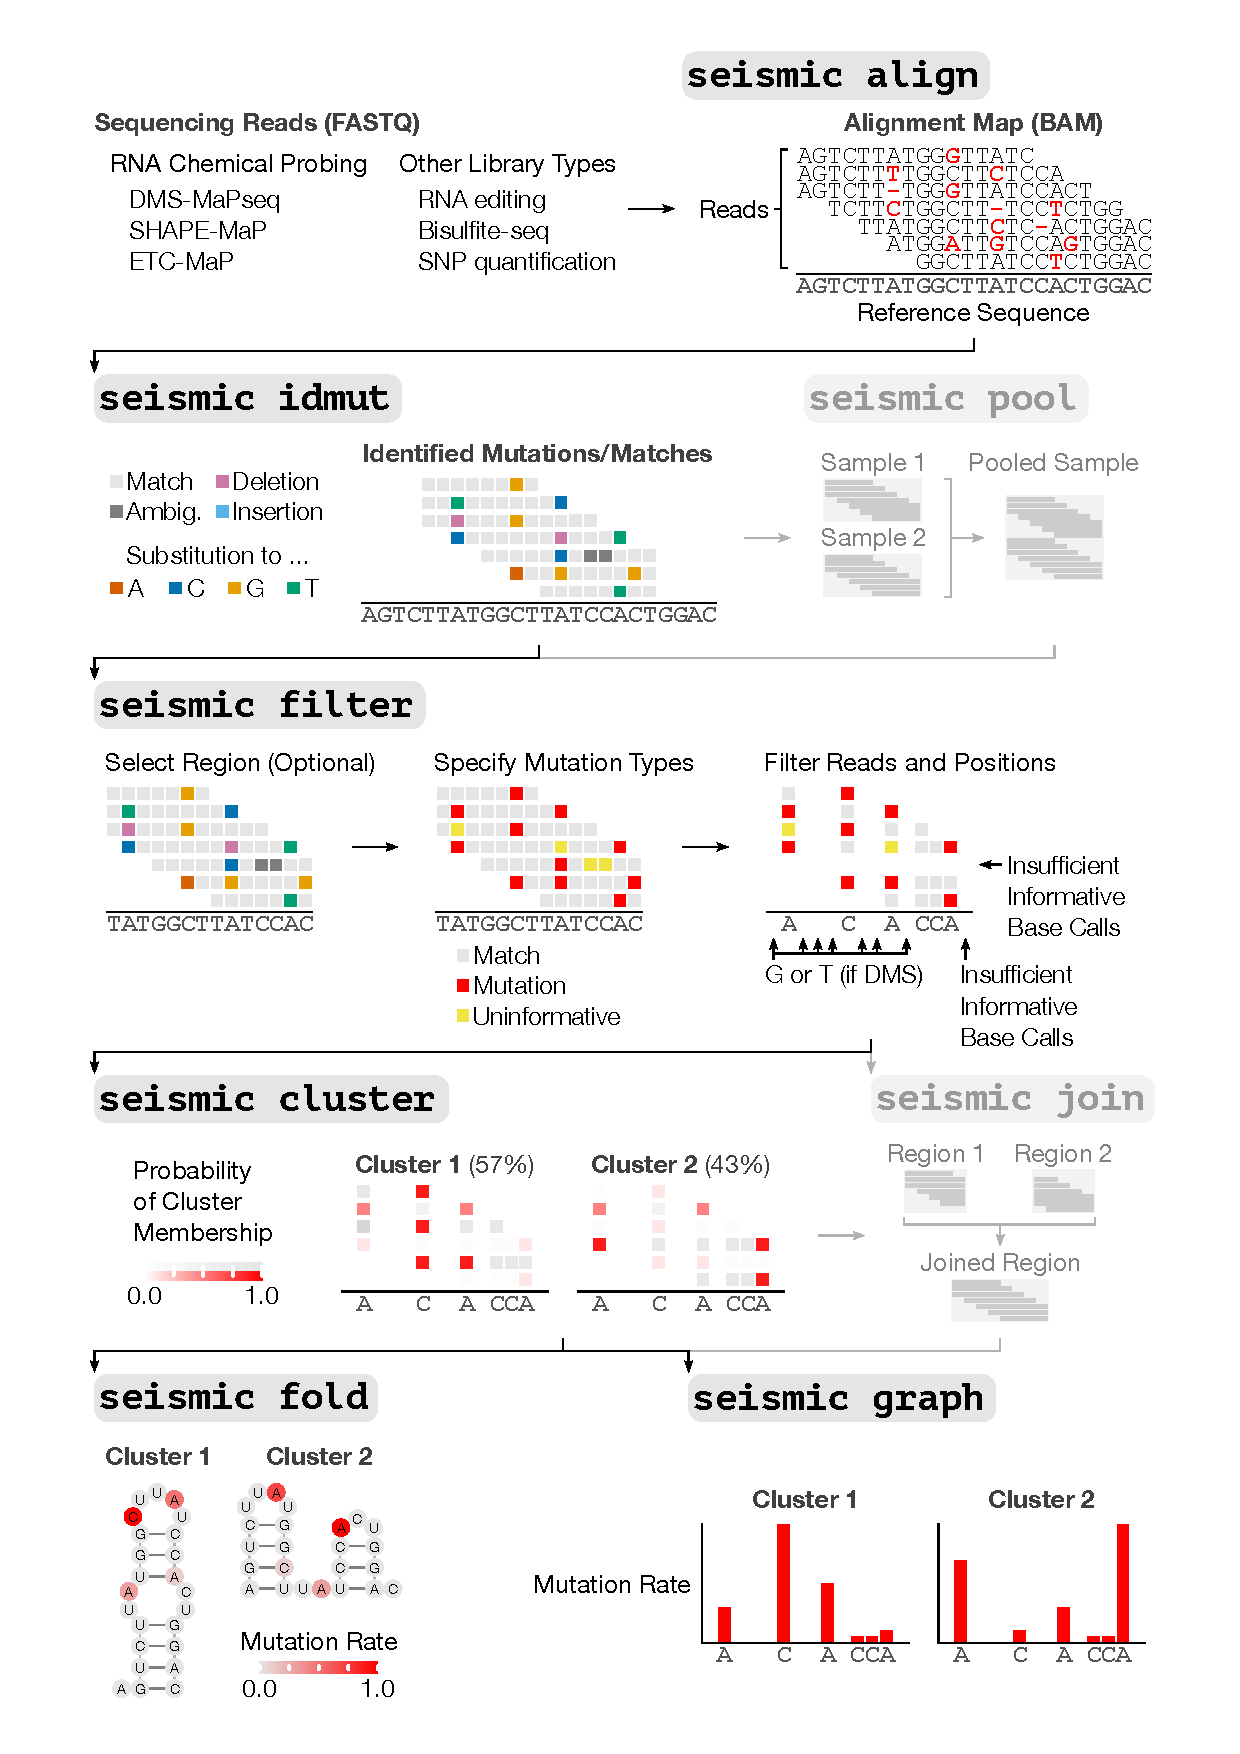
\includegraphics[width=0.95\textwidth]{Figure_1.pdf}
    \caption{\textbf{SEISMIC-RNA processes sequencing reads into predicted RNA structures.} (Continued on next page.)}
    \label{wf}
\end{figure*}
\addtocounter{figure}{-1}
\pagebreak
\begin{figure*}[!t]
    \caption[]{(Continued from previous page.) As input, SEISMIC-RNA accepts sequencing reads from RNA mutational profiling experiments (e.g. DMS-MaPseq~\cite{Zubradt2016} , SHAPE-MaP~\cite{Siegfried2014}, ETC-MaP~\cite{Douds2024}) or other experiments whose readouts are point mutations. SEISMIC-RNA first aligns the reads to the reference sequence of each RNA using Bowtie~2~\cite{Langmead2012}. Next, it determines the relationship (i.e. match, substitution, deletion, insertion) between each read and each position in the reference. It marks low-quality base calls and deletions/insertions in repetitive sequences as ambiguous. It also clips 4 bases from both ends of each read to correct bias against mutations during local alignment. Optionally, users can then pool together multiple samples, such as replicates. Next, SEISMIC-RNA selects relevant data and filters out the remainder: users optionally select a region of the RNA to analyze, specify which relationships to count as mutations, and filter out unusable reads and positions. SEISMIC-RNA then clusters the remaining data to detect alternative RNA structures. Every read is assigned a probability of belonging to each cluster; for each cluster, its proportion is the average of all read probabilities, and its mutation rates are the probability-weighted averages over all reads. Optionally, users can join multiple regions that were filtered or clustered individually. SEISMIC-RNA can then use the mutation rates to predict the RNA structure corresponding to each cluster using RNAstructure~\cite{Reuter2010}, as well as generate graphs, such as bar graphs of the mutation rates. This entire workflow (except pool and join) can be run with one command: \texttt{seismic wf}.}
\end{figure*}
\pagebreak


\begin{figure*}[!t]
    \centering
    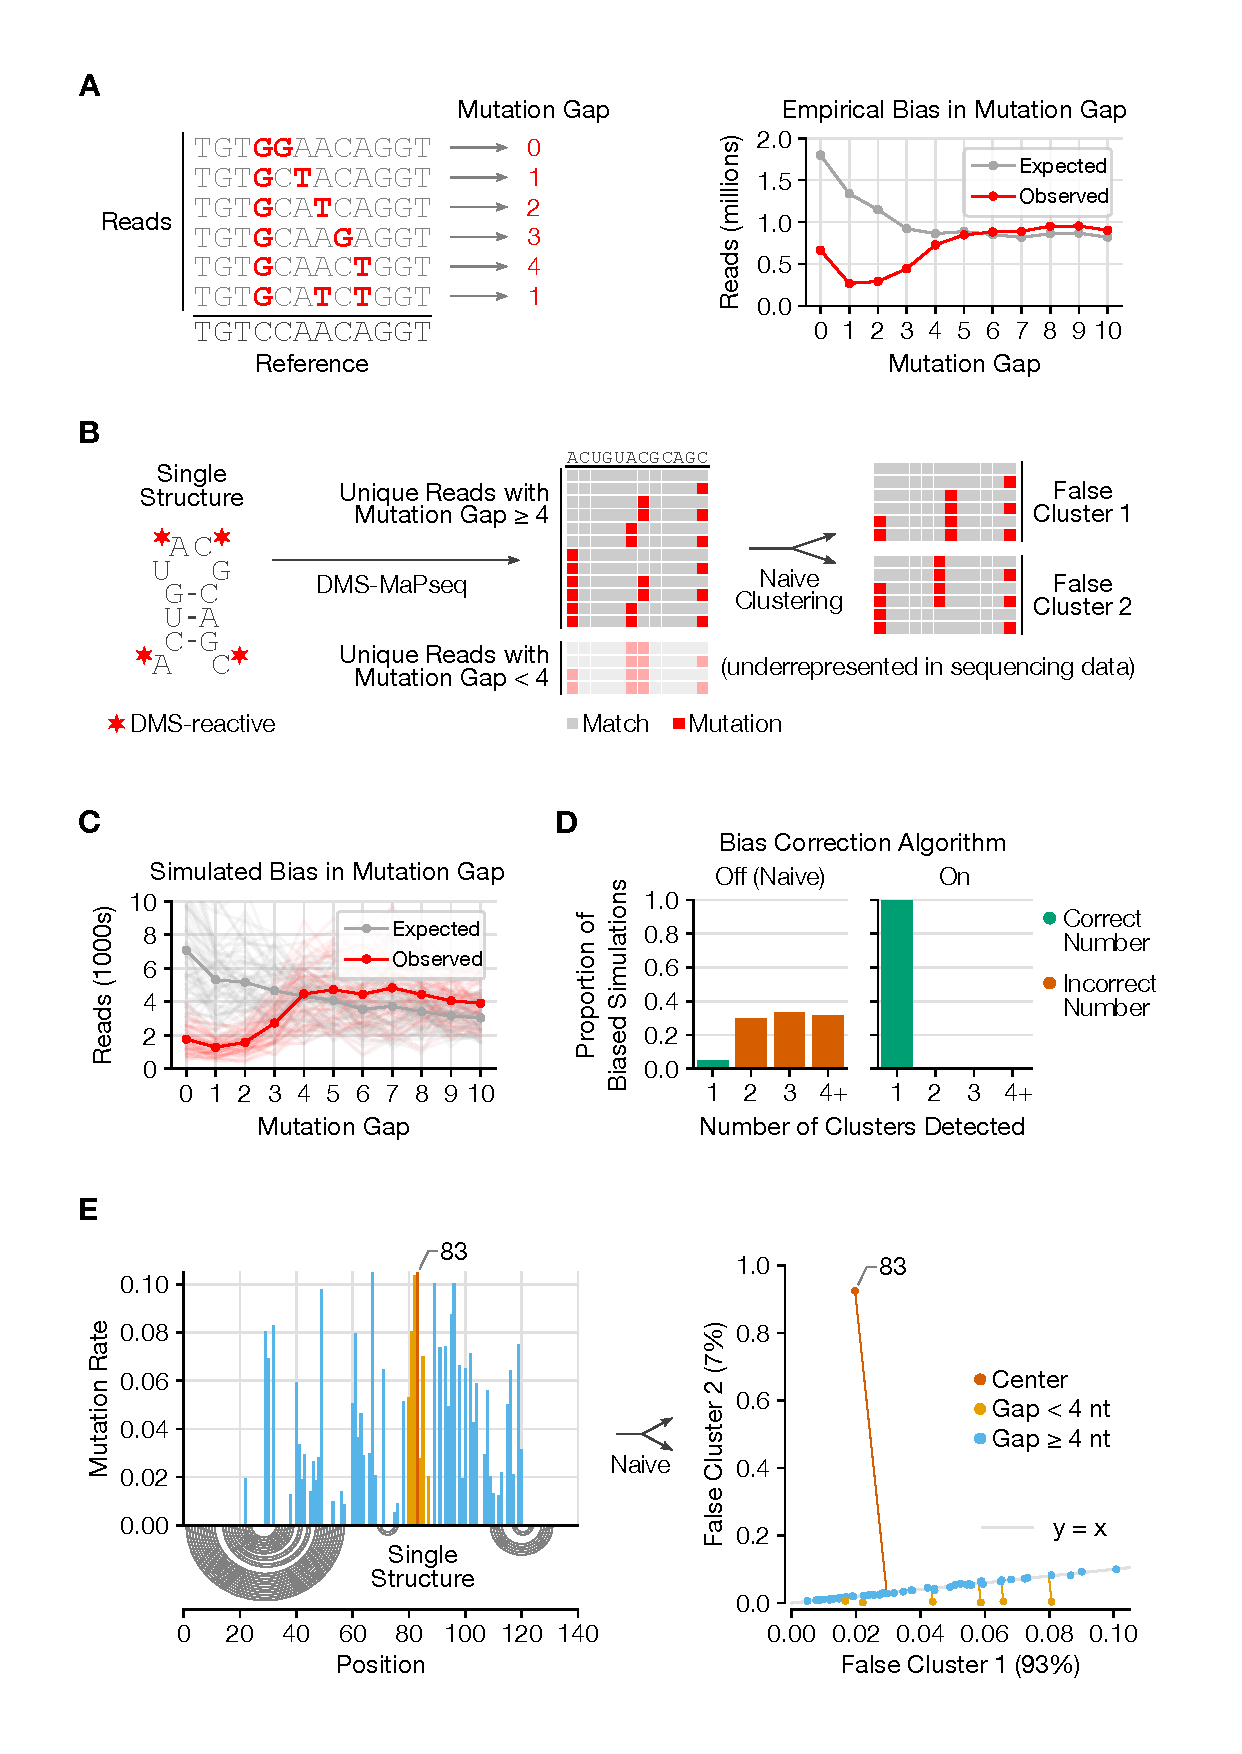
\includegraphics[width=0.95\textwidth]{Figure_2.pdf}
    \caption{\textbf{Reads with nearby mutations are underrepresented, producing false clusters unless corrected for.} (Continued on next page.)}
    \label{mutation-gap}
\end{figure*}
\addtocounter{figure}{-1}
\pagebreak
\begin{figure*}[!t]
    \caption[]{(Continued from previous page.) \textbf{(A)} Reads whose two closest mutations have a gap less than 4~nt are underrepresented in DMS-MaPseq data~\cite{Morandi2021} compared to the theoretical expectation if mutations occurred independently. \textbf{(B)} Underrepresentation of reads with nearby mutations can cause false clusters. For an RNA that forms a single structure, reads with two mutations less than 4~nt apart will occur rarely in sequencing data. Thus, the two mutations will be anti-correlated, so a naive clustering algorithm will falsely create a cluster for each mutation. \textbf{(C)} We simulated DMS-MaPseq data for 60 random RNA sequences, each with one true cluster, to have bias similar to that of empirical data. Each light trace represents one simulated dataset; the dark traces are the average of all simulated datasets. \textbf{(D)} Without correcting for the bias in mutation gaps, 95\% of simulated datasets incorrectly yielded more than one cluster. With SEISMIC-RNA's bias correction algorithm, all datasets correctly yielded one cluster. \textbf{(E)} In a representative RNA that yielded two clusters without bias correction, position 83 (red) is one of the most frequently mutated positions and is surrounded by six other positions with mutation rates of at least 2\% (orange). Clustering without bias correction assigned reads in which position 83 was mutated predominantly to cluster 2, and reads in which any surrounding position was mutated predominantly to cluster 1, in agreement with panel (B).}
\end{figure*}

\begin{figure*}[!t]
    \centering
    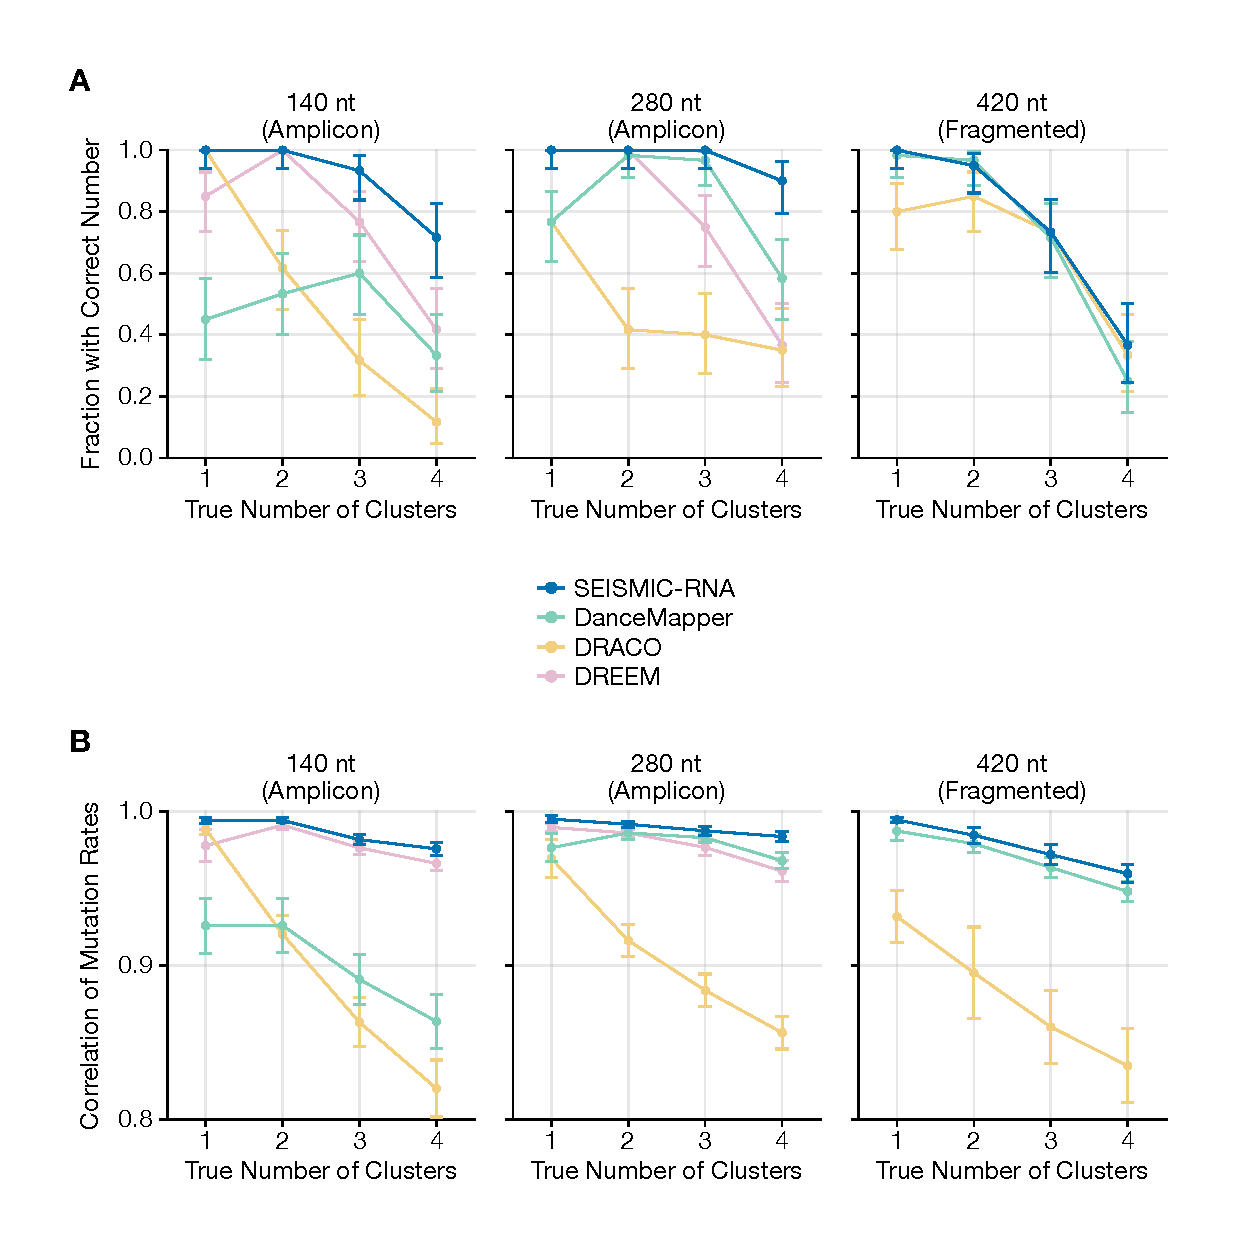
\includegraphics[width=0.95\textwidth]{Figure_3.pdf}
    \caption{\textbf{SEISMIC-RNA is more accurate than similar software.} \textbf{(A)} The fraction of 60 simulations for which SEISMIC-RNA, DanceMapper, DRACO, and DREEM detected the correct number of clusters for each length of RNA and true number of clusters. Error bars show 95\% confidence intervals. \textbf{(B)} The average Pearson correlation between the true mutation rates and those calculated by SEISMIC-RNA, DanceMapper, DRACO, and DREEM for each length of RNA and true number of clusters. Error bars show 95\% confidence intervals.}
    \label{accuracy}
\end{figure*}

\begin{figure*}[!t]
    \centering
    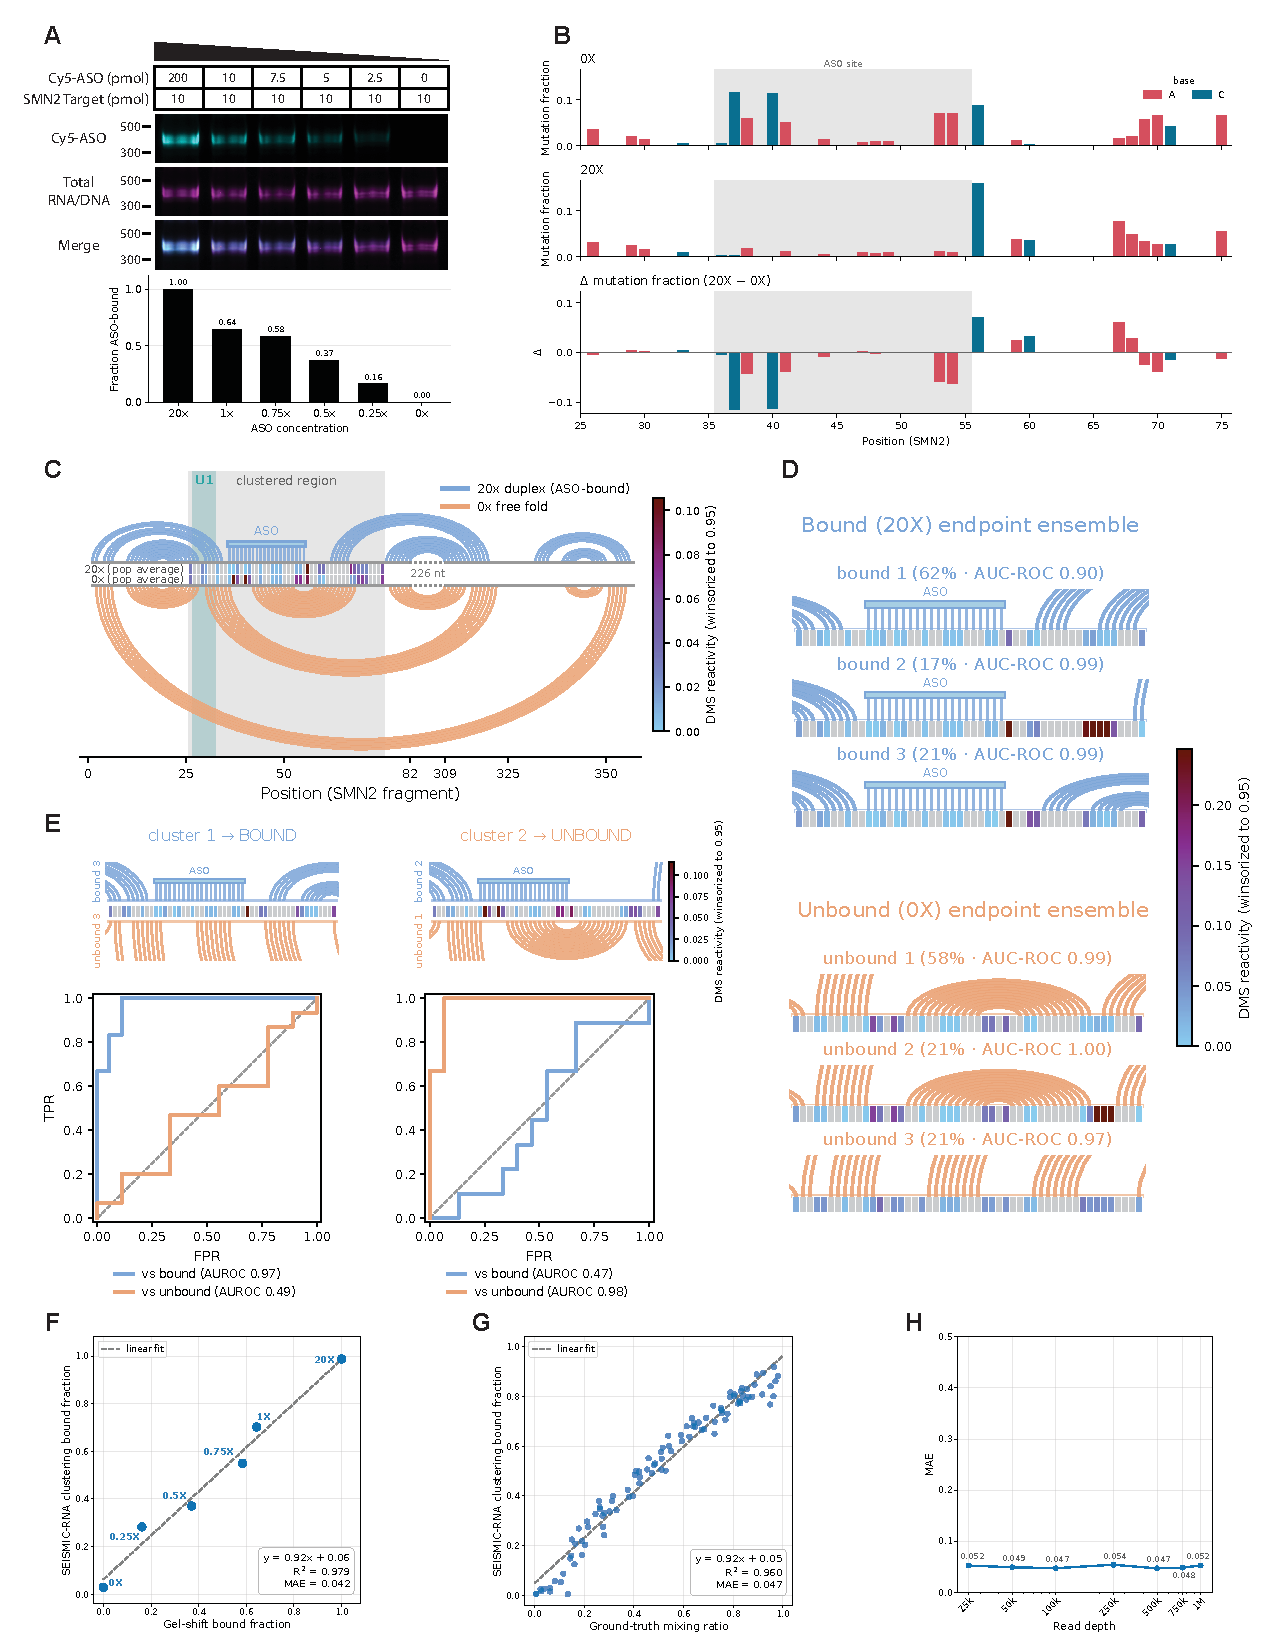
\includegraphics[width=0.95\textwidth]{Figure_4.pdf}
    \caption{\textbf{The SEISMIC-RNA duplex module enables accurate quantification of ASO binding from experimental data.} \textbf{(A)} Native gel-shift titration of a Cy5-labeled ASO folded with a fixed amount of the \textit{SMN2} target RNA fragment. Top: fluorescence scans of Cy5-ASO, total RNA/DNA, and their merge over decreasing ASO input. Bottom: intensity of the shifted Cy5-ASO band normalized to total RNA/DNA loading and the saturating 20X condition, i.e. the fraction of target bound to ASO. \textbf{(B)} Population-average DMS reactivity after processing and filtering with SEISMIC-RNA for the unbound (0X) and saturated (20X) samples, and their difference ($\Delta$, 20X $-$ 0X). The ASO binding region is shaded in gray. (Continued on next page.)}
    \label{aso}
\end{figure*}
\addtocounter{figure}{-1}
\pagebreak
\begin{figure*}[!t]
    \caption[]{\textbf{(C)} Arc diagrams of the representative endpoint secondary structures generated from the population-average DMS data over the whole \textit{SMN2} fragment. The 20X model (top, blue) was cofolded with the ASO sequence using the \texttt{seismic duplex} module. The 0X model (bottom, orange) was generated directly from the filtered data with \texttt{seismic fold}. The intervening 226~nt of the reported long-range interaction are collapsed, and the central heatmap shows the winsorized population-average DMS reactivities from \textbf{B}. The U1 snRNP binding site and the clustered region (positions 26-75) are shaded. \textbf{(D)} Endpoint reference clusters and their constrained structures used for assignment of bound and unbound fractions. Each panel shows the cluster reactivities and the representative (highest AUC-ROC) structure folded using reactivities over the clustered region only. Top, blue: the three detected 20X clusters and their structures generated with the \texttt{seismic duplex} module. Bottom, orange: the three detected 0X clusters and their structures generated directly with \texttt{seismic fold}. The cluster abundance and AUC-ROC are noted in the cluster label. \textbf{(E)} Example AUC-ROC--based assignment of clusters to the bound or unbound state. The DMS reactivities of clusters from a mixed sample (computational mixture, 100k read pairs) are compared against the best-scoring AUC-ROC structures from each endpoint ensemble in \textbf{D}. Cluster 1's reactivities (left heatmap) fit the best bound structure (blue curve, AUC-ROC 0.97) better than the best unbound structure (orange curve, AUC-ROC 0.49), causing the cluster to be assigned as bound. Cluster 2's reactivities (right heatmap) fit the best unbound structure (orange curve, AUC-ROC 0.98) better than the best bound structure (blue curve, AUC-ROC 0.47), causing the cluster to be assigned as unbound. \textbf{(F)} SEISMIC-RNA cluster-derived bound fractions versus the gel-shift ground truth across the six-point ASO titration. \textbf{(G)} One hundred computational mixtures of 0X and 20X reads at random bound fractions (100k read pairs each) scored against the ground-truth mixing ratio as in \textbf{F}. \textbf{(H)} The MAE of SEISMIC-RNA's clustering of computational mixtures against the ground-truth mixing ratios is stable for the \textit{SMN2} ensemble over read depths spanning from 25k to 1M. TPR: True Positive Rate, FPR: False Positive Rate, MAE: Mean Absolute Error.}
\end{figure*}

\begin{figure*}[!t]
    \centering
    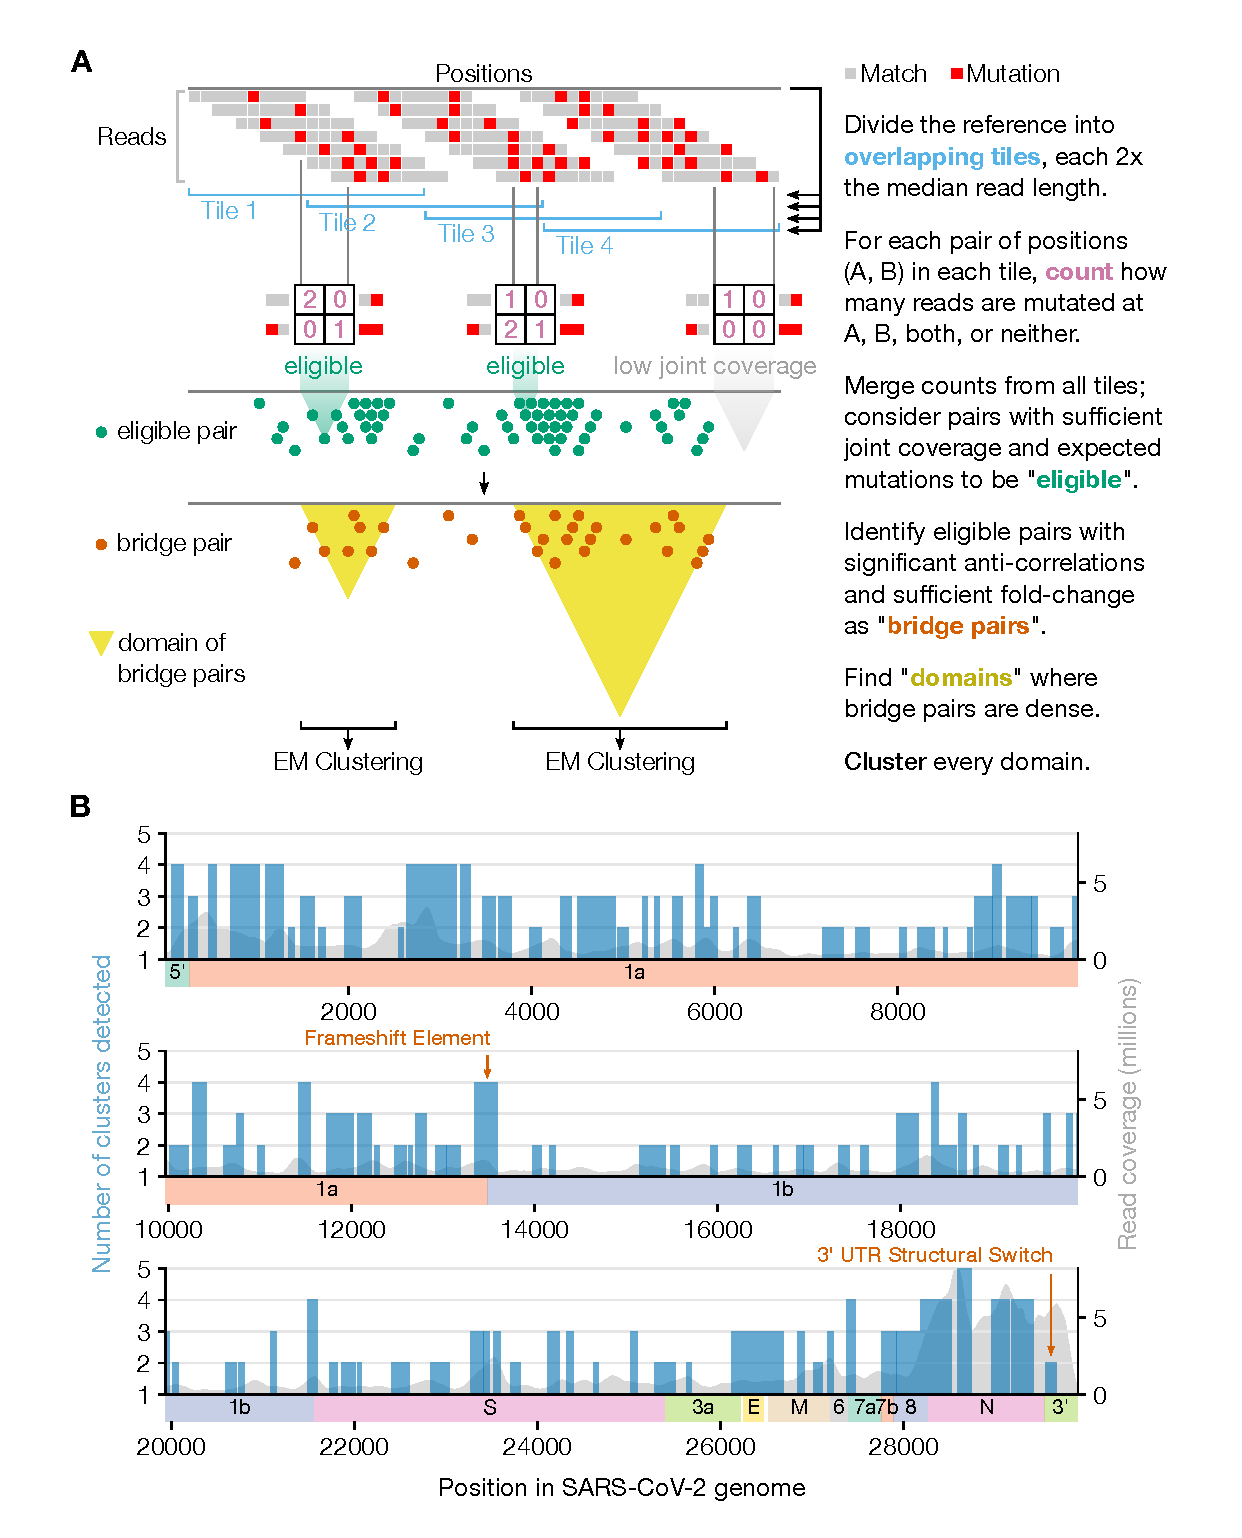
\includegraphics[width=0.95\textwidth]{Figure_5.pdf}
    \caption{\textbf{SEISMIC-RNA clusters long transcripts by first identifying domains that form multiple clusters.} \textbf{(A)} First, SEISMIC-RNA divides a long transcript into tiles (light blue), each twice the median read length and overlapping at least half of each adjacent tile. For each pair of positions (A, B) in each tile, it counts how many reads cover both positions and have A and B both mutated, only A mutated, only B mutated, or neither mutated ($2 \times 2$ matrices, purple). Counts from all tiles are merged into one table; a pair found in more than one tile keeps the counts from the tile in which it has the greatest joint coverage. Then pairs of positions with sufficient joint coverage (default 1,000) and sufficient expected joint mutations (default 5.0) are deemed ``eligible" (green). Eligible pairs with statistically significant anti-correlations and sufficient fold-change in joint mutated count relative to the expectation under independence are deemed ``bridge pairs" (red). It then identifies regions called ``domains" where bridge pairs are most dense using a dynamic programming algorithm. Finally, it clusters each domain, and optionally each gap between domains. \textbf{(B)} Scanning clustering analysis of the SARS-CoV-2 genome using data from Morandi et al.~\cite{Morandi2021}. Each domain identified by SEISMIC-RNA that formed at least 2 clusters is represented by a blue bar whose x coordinates indicate the beginning and end of the domain and whose height indicates the number of clusters (left y axis). The read coverage (as a moving average over 121~nt windows) is shown as a light gray fill (right y axis). The 5' and 3' UTRs and each open reading frame (ORF), based on the annotation for \texttt{NC\_045512.2} but without ORF10 are drawn below the x axis. Two elements known to form multiple structures -- the Frameshift Element and the 3' UTR structural switch -- are labeled in red.}
    \label{ensembles}
\end{figure*}


\end{document}
